\documentclass[a4paper,10pt,oneside]{book}
\usepackage[utf8]{inputenc}
\usepackage[italian]{babel}
\usepackage[T1]{fontenc}
\usepackage{lmodern}
\usepackage{hyperref}
\usepackage{mathtools}				% Matematica
\usepackage{microtype}				% Microgiustificazione
\usepackage{makeidx}				% indice analitico
\usepackage{hyperref}				% Gestione riferimenti incrociati
\usepackage{amssymb}				% Simboli matematici
\usepackage{wasysym}
\usepackage{mathcomp}
\usepackage{amsmath}
\usepackage{pifont}

\title{Elaborazione e Analisi delle Immagini}
\author{Giuseppe Bellisano}
\date{}

\makeindex

\usepackage[nonumberlist]{glossaries} % glossario
%\glossarystyle{altlisthypergroup}
	\makeglossaries
	
\newglossaryentry{trasformazione geometrica affine}
{
	name=trasformazione geometrica affine, description={Esempi di affinità sono rotazioni, omotetie, traslazioni, rototraslazioni, riflessioni. Le affinità non sono necessariamente isometrie, non preservano cioè angoli e distanze, mentre mantengono sempre il parallelismo tra le rette.}
}
% --------------------------------------------------------------------
\newglossaryentry{omega}{%
	name=insieme connesso2,
	description={pulsazione naturale2},
}
% --------------------------------------------------------------------
\newglossaryentry{connesso}{%
	name=connesso,
	description={pulsazione naturale},
}
% --------------------------------------------------------------------
\newglossaryentry{omega2}{%
	name=$\omega_\mathrm{n}$,
	description={pulsazione naturale},
}
% --------------------------------------------------------------------
\newglossaryentry{Region growing}{%
	name=regionGrowing,
	description={Region growing (traducibile in italiano come "accrescimento delle regioni") è un semplice metodo di segmentazione di immagini basato su regioni. Viene anche considerato come un metodo basato sul singolo pixel poiché tale metodo comporta inizialmente la selezione dei punti seme. Questo approccio alla segmentazione esamina i pixel adiacenti di punti iniziali, detti semi, e determina se i vicini di pixel possono essere aggiunti a tale regione. Il processo viene iterato, allo stesso modo come negli algoritmi di clustering di dati.},
}

\usepackage{listings}
\usepackage{color}
\definecolor{mygreen}{rgb}{0,0.6,0}
\definecolor{mygray}{rgb}{0.5,0.5,0.5}
\definecolor{mymauve}{rgb}{0.58,0,0.82}

\lstset{ %
  backgroundcolor=\color{white},   % choose the background color; you must add \usepackage{color} or \usepackage{xcolor}; should come as last argument
  basicstyle=\footnotesize,        % the size of the fonts that are used for the code
  breakatwhitespace=false,         % sets if automatic breaks should only happen at whitespace
  breaklines=true,                 % sets automatic line breaking
  captionpos=b,                    % sets the caption-position to bottom
  commentstyle=\color{mygreen},    % comment style
  deletekeywords={...},            % if you want to delete keywords from the given language
  escapeinside={\%*}{*)},          % if you want to add LaTeX within your code
  extendedchars=true,              % lets you use non-ASCII characters; for 8-bits encodings only, does not work with UTF-8
  frame=single,	                   % adds a frame around the code
  keepspaces=true,                 % keeps spaces in text, useful for keeping indentation of code (possibly needs columns=flexible)
  keywordstyle=\color{blue},       % keyword style
  language=Matlab,                 % the language of the code
  morekeywords={*,...},           % if you want to add more keywords to the set
  numbers=left,                    % where to put the line-numbers; possible values are (none, left, right)
  numbersep=5pt,                   % how far the line-numbers are from the code
  numberstyle=\tiny\color{mygray}, % the style that is used for the line-numbers
  rulecolor=\color{black},         % if not set, the frame-color may be changed on line-breaks within not-black text (e.g. comments (green here))
  showspaces=false,                % show spaces everywhere adding particular underscores; it overrides 'showstringspaces'
  showstringspaces=false,          % underline spaces within strings only
  showtabs=false,                  % show tabs within strings adding particular underscores
  stepnumber=2,                    % the step between two line-numbers. If it's 1, each line will be numbered
  stringstyle=\color{mymauve},     % string literal style
  tabsize=2,	                   % sets default tabsize to 2 spaces
  title=\lstname                   % show the filename of files included with \lstinputlisting; also try caption instead of title
}

\begin{document}
\maketitle
\tableofcontents 					%indice generale

\chapter{Immagini}

\section{Image processing, analysis e understanding. Spiegarne la differenza}

Abbiamo tre categorie principali di manipolazione delle immagini:
\begin{itemize}
\item \textbf{image processing} (input: immagine -> output: immagine);
\item \textbf{image analysis} (input: immagine -> output: metriche);
\item \textbf{image understanding} (input: immagine -> output: descrizione ad alto livello)
\end{itemize}

Nell'\textbf{image processing} l'input della manipolazione è un'immagine e l'output è ancora un'immagine e più precisamente si tratta dell'immagine originale opportunamente processata (grazie a tecniche di miglioramento e rimozione del rumore)

Nell'\textbf{image analysis} è la trasformazione che fa passare dall’immagine a una sua rappresentazione astratta, cioè ad una sua descrizione ad alto livello

Nell'\textbf{image understanding} data un'immagine otteniamo invece descrizioni di alto livello sul contenuto dell'immagine (ad esempio il riconoscimento degli oggetti all'interno delle immagini e le relazioni tra di essi).

\section{Definire una immagine digitale}
Un'immagine digitale è una rappresentazione numerica/digitale di un'immagine attraverso una matrice rettangolare, in cui ad ogni posizione (che prende il nome di pixel) sono assegnati uno o più valori numerici e ad ogni posizione corrisponde una coordinata reale sul piano immagine. 

\subsection{Dettagli}
Perché le immagini siano elaborate al computer occorre trasformarle in una rappresentazione numerica/digitale attraverso un processo chiamato digitalizzazione. 

Le immagini digitali sono matrici rettangolari in cui ad ogni posizione corrispondono uno o più valori numerici: ad ogni posizione corrisponde una coordinata reale sul piano immagine; ogni punto prende il nome di pixel (picture per element).

Un immagine digitale f[m,n] descritta in uno spazio discreto 2D è derivata da un immagine analogica f(x,y) in uno spazio continuo 2D attraverso il processo di campionamento (sampling) detto digitalizzazione. L'immagine continua in 2D f(x,y) viene divisa in N righe ed M colonne.

L'intersezione di una riga con una colonna determina un pixel. Il valore assegnato alle coordinate intere [m,n] con {m = O, 1, 2,..., M-1} e {n = O, 1, 2,..., N-1} è f[m,n]. e rappresenta l'intensità di grigio associata al punto identificato. Il numero dei valori di grigi generalmente è una potenza di 2: L=2 B (se B>1 si parla di immagine in scala di grigi, se B=1 si parla di immagini binarie).

Quando un'immagine viene digitalizzata il sampling avviene sia a livello spaziale (con le righe e le colonne) sia a livello di ampiezza (con la quantizzazione dei livelli di grigio).

\section{Cosa si intende per risoluzione di una immagine?}
La risoluzione è un indice della qualità di un'immagine. E' la quantità dei suoi punti elementari (pixel) rapportata ad un'unità di lunghezza, dove quest'ultima di solito è il pollice (dpi, dot per inch).

\subsection{Dettagli}
Possiamo distinguere due tipi di risoluzione: spaziale e dei livelli d'intensità.
\begin{itemize}

\item \textbf{La risoluzione spaziale} indica il più piccolo dettaglio distinguibile nell'immagine. È quindi una misura della densità dei pixel di un'immagine (che si misura in punti per unità di lunghezza, che solitamente è il pollice).

Poiché un'immagine digitale è discreta ed è rappresentata come un insieme di punti, se il numero di punti per unità di lunghezza è molto elevato, allora ogni pixel rappresenta dettagli più piccoli e quindi aumentando il numero di pixel aumento il dettaglio percepito dall'occhio umano.

La risoluzione spaziale è quindi strettamente dipendente dalla frequenza di campionamento dell'immagine digitale.

\item \textbf{La risoluzione dei livelli d'intensità}, in modo simile,  consiste nel più piccolo cambiamento del livello d'intensità distinguibile nell'immagine. Anche in questo caso se l'immagine presenta un elevato numero di livelli d'intensità differenti, allora la risoluzione sarà maggiore, in quanto non verrà percepito il passaggio da un livello all'altro. La risoluzione dei livelli d'intensità è quindi legata alla frequenza di campionamento in ampiezza (quantizzazione dei livelli d'intensità) dell'immagine.

La quantizzazione (campionamento in ampiezza) può essere uniforme, ovvero le intensità degli oggetti sono mappate in modo diretto sui livelli di grigio dell'immagine, oppure può essere logaritmica (maggior risoluzione nelle zone scure). L'occhio umano ha una percezione logaritmica dei livelli di grigio.

La scelta del campionamento viene fatta in base all'uso dell'immagine, alle limitazioni della memoria e della velocità dell'elaborazione, alla necessità o meno di analizzare l'immagine e alle informazioni che bisogna estrarne.
\end{itemize}

\section{Illustrare il processo di campionamento e quantizzazione}
La digitalizzazione di un'immagine comprende il campionamento e la quantizzazione. Sono entrambi processi di discretizzazione. Il campionamento consiste nella discretizzazione del dominio spaziale e in genere è uniforme, mentre la quantizzazione consiste nella discretizzazione dei livelli di grigio e può essere sia uniforme che logaritmica.

\subsection{Dettagli}
Quando un immagine viene digitalizzata, il campionamento (sampling) avviene sia a livello spaziale (con le righe e le colonne) sia a livello di ampiezza (con la quantizzazione dei livelli di grigio).

Per campionare un'immagine è necessario scegliere innanzitutto quanti pixel vogliamo rappresentare (campionamento spaziale), scegliendo quindi il numero di righe e di colonne della matrice che rappresenterà l'immagine. Da questa scelta dipenderà ovviamente la risoluzione dell'immagine digitalizzata.

\begin{itemize}
\item Il sampling spaziale può essere uniforme, ovvero il campionamento ha la stessa frequenza su tutta l'immagine, oppure adattivo ovvero si utilizza maggiore frequenza nelle aree con più dettaglio. Il valore discreto frutto del sampling si chiama pixel (picture element) nello spazio 2D e voxel (volume element) nello spazio 3D.

\item La risoluzione indica il più piccolo dettaglio ottenibile dall'immagine. La frequenza di campionamento limita la risoluzione.
La quantizzazione dei livelli di luminosità dei pixel (ossia il campionamento in ampiezza) consiste invece nel decidere il numero di valori di intensità rappresentabili per ogni pixel (che solitamente è una potenza di 2).

\item La quantizzazione (campionamento in ampiezza) può essere uniforme, ovvero le intensità degli oggetti sono mappate in modo diretto sui livelli di grigio dell'immagine, oppure può essere logaritmica (maggior risoluzione nelle zone scure). L'occhio umano ha una percezione logaritmica dei livelli di grigio.
La scelta del campionamento viene fatta in base all'uso dell'immagine, alle limitazioni della memoria e della velocità dell'elaborazione, alla necessità o meno di analizzare l'immagine e alle informazioni che bisogna estrarne.

\item Le immagini a colori contengono maggiori informazioni di quelle monocromatiche. L'uomo rileva i colori come una combinazione dei tre colori primari: rosso, verde e blu. Il computer usa quindi il modello RGB in cui un pixel può essere associato ad un vettore tridimensionale che fornisce le
rispettive intensità dei tre colori; abbiamo quindi ad esempio: nero= (O,O,O); bianco=(k-1,k-1,k-1); rosso puro=(k-1,O,O) dove k è il range di intensità possibile (quindi i colori rappresentabili col modello RGB sono $k^3$).

Un altro modo per rappresentare le immagini a colori è il modello HSL (hue = tonalità, saturation = saturazione, lightness = luminosità) simile al modello RGB nel funzionamento.
\end{itemize}

\section{Descrivere i passi fondamentali di un processo di elaborazione di immagini digitali}
I passi fondamentali di un processo di elaborazione di immagini digitali sono quattro:
\begin{itemize}

\item \textbf{Acquisizione dell'immagine}: consiste nella digitalizzazione dell'immagine da elaborare, ossia il processo di campionamento con cui si cerca di derivare da un'immagine reale, definita nello spazio continuo, un'immagine discreta, rappresentabile come matrice. In questa fase avviene quindi la scelta del campionamento spaziale e in ampiezza da cui dipende la risoluzione dell'immagine.

\item \textbf{Preprocessing}: comprende tutte quelle operazioni di basso livello che si eseguono sulle immagini. Lo scopo è quello di enfatizzare una certa caratteristica allo scopo di rendere più adatta l'immagine a computazioni future di livello più alto. Esempi tipici sono il miglioramento del contrasto, lo smoothing, correzione di distorsioni, eliminazione del rumore.

\item \textbf{Segmentazione}: consiste nella suddivisione di un'immagine in modo da identificare ed isolare gli oggetti che compaiono nell'immagine stessa. È uno degli aspetti più complicati del processo di elaborazione delle immagini digitali.

\item \textbf{Descrizione e classificazione degli oggetti ottenuti dalla segmentazione}: con metodi ad alto livello si possono ricavare informazioni e modelli (image
understanding, visione) e a trovare le relazioni tra di essi (ad esempio la posizione di un oggetto rispetto ad un altro).
\end{itemize}

\section{Dettagli}
L'elaborazione di immagini digitali è una disciplina che definisce tecniche e algoritmi informatici per modificare immagini digitali allo scopo di: migliorarne la qualità (riduzione del rumore o aumento del contrasto); generare codifica utile, compressione; generare visualizzazioni (grafica computazionale); estrarre semplici features; ricavare informazioni/modelli (image understanding, visione).

La Computer Vision mira a riprodurre l'effetto della vista umana utilizzando la percezione elettronica di un'immagine e la sua successiva comprensione. Possiamo distinguere due livelli: High Level Image Understanding e Low Level Image Processing.
\begin{itemize}
	\item il processing di basso livello utilizza poche informazioni riguardo il contenuto dell'immagine
	\item il processing di alto livello fa l'esatto opposto: utilizza tali informazioni per cercare di simulare le capacità cognitive umane e la nostra abilità nel prendere decisioni in base a ciò che l'immagine rappresenta. Per fare questo spesso nel processing di alto livello si ricorre a tecniche tipiche dell'intelligenza artificiale.
\end{itemize}

La vista umana non dà un'immagine fedele del mondo esterno ma ne dà un'interpretazione spesso fallace. Questo perché il cervello umano tende ad associare le informazioni in insiemi correlati sulla base di: raggruppamento, somiglianza, continuità, chiusura, figura/sfondo, profondità, costanza forme in prospettiva e moto.
La visione umana è un processo di interpretazione molto complesso, ma in qualche modo computazionale. Si basa su informazioni a priori, innate ed acquisite. Difficilmente imitabile da un sistema artificiale. Sono imitabili però alcune idee e procedure. Il computer invece misura valori assoluti, esegue calcoli ed è: instancabile, economico, veloce e oggettivo.

\chapter{Concetti base sulle immagini digitali}

\section{Come si classificano le operazioni spaziali da applicare su un'immagine digitale?}
I tipi di operazioni che possono essere applicati ad immagini digitali per trasformare un'immagine input $a[M,N]$ in un'immagine output $b[M,N]$ (o altre rappresentazioni) possono essere classificate in tre categorie:
\begin{itemize}

\item \textbf{Puntuali}: il valore di output ad una specifica coordinata dipende solo dal valore in input alla medesima coordinata. La complessità associata a questo tipo di operazioni è costante

\item \textbf{Locali}: il valore di output ad una specifica coordinata dipende non solo dall'input del valore alla medesima coordinata ma anche da un suo intorno. La complessità è quadratica sulle dimensioni dell'intorno scelto

\item \textbf{Globali}: il valore di output ad una specifica coordinata dipende da tutti i valori dell'immagine input. La complessità è quadratica sulle dimensioni dell'immagine stessa
\end{itemize}

\section{Definire il concetto di adiacenza nelle immagini digitali}
L'adiacenza è quella relazione fra due pixel di un'immagine digitale per cui la loro distanza è uguale a 1. 
\begin{itemize}

	\item \textbf{City Block}
	La distanza City Block da un dato pixel è dato da tutti quei pixel che hanno distanza 1 (dal suddetto pixel) compiendo un solo passo in verticale o in orizzontale
(4-adiacenza)

	\item \textbf{Scacchiera (Chessboard)}
	La distanza Scacchiera (Chessboard da un dato pixel è dato da tutti quei pixel che hanno distanza 1 (dal suddetto pixel) compiendo un solo passo in verticale, in orizzontale o anche in diagonale (8-adiacenza)
\end{itemize}

\section{Definire una regione di un'immagine binaria}
Una regione è un insieme connesso di pixel in cui esiste un percorso fra ogni coppia di questi pixel. Questo percorso è tracciato saltando sempre da un pixel al pixel adiacente, e ciascuno di questi pixel appartiene alla regione.
Una regione può avere buchi al suo interno.

\section{Definire un contorno in un'immagine binaria}
\begin{itemize}
	\item il bordo interno è l'insieme dei pixel di una regione che hanno almeno un pixel adiacente non	appartenente alla regione
	\item il bordo esterno è invece costituito dai pixel esterni alla regione che hanno almeno un pixel adiacente appartenente alla regione
\end{itemize}

\section{Definire un edge in un'immagine digitale}
Formalmente l'edge è una proprietà di un pixel e del suo intorno. In un'immagine digitale, è detto "di edge" un pixel nel cui intorno sono presenti dei pixel con livelli di grigio che variano bruscamente.

\section{Illustrare il concetto di distanza tra punti in una immagine digitale}
La distanza tra punti di coordinate (i, j) e (h, k) può essere definita come distanza:
\begin{itemize}
	\item \textbf{Euclidea} $D_e[(i,j), (h,k)] = \sqrt{(i - h)^2 + (j - k)^2}$ 
	
	\item \textbf{City Block} $D_4[(i,j), (h,k)] = |i - h| + |j - k|$
	La distanza City Block da un dato pixel è dato da tutti quei pixel che hanno distanza 1 (dal suddetto pixel) compiendo un solo passo in verticale o in orizzontale
	
	\item \textbf{Scacchiera (Chessboard)} $D_8[(i,j), (h,k)] = max\{|i - h|, |j - k| \}$
	La distanza Scacchiera (Chessboard da un dato pixel è dato da tutti quei pixel che hanno distanza 1 (dal suddetto pixel) compiendo un solo passo in verticale, in orizzontale o anche in diagonale
\end{itemize}

\section{Fornire la definizione di istogramma di un'immagine}
L'istogramma di un'immagine digitale $f[m,n]$ è una funzione che a ciascun livello di grigio definito nella quantizzazione dell'immagine, fa corrispondere un valore pari al numero di pixel dell'immagine a cui è assegnato quel livello di grigio.
$$
H(k) = card \{ f(x,y) | f(x,y) = k \}
$$ 

con $k = 0, 1, \dots, 2^{B}-1$ 

per cui vale: 
$$ 
\displaystyle\sum_{k=0}^{{2^B}-1} H(k) = M \cdotp N
$$

dove $card = \#$

\subsection{Dettagli}
Le immagini a colori hanno tre istogrammi: uno per ogni componente. 

Ecco un esempio di istogramma per un'immagine monocromatica 4x4 a 3 bit:
$$
\begin{array}{c|c|c|c}
	6 & 7 & 3 & 3 \\ 
	\hline
	2 & 6 & 1 & 0 \\
	\hline
	4 & 6 & 1 & 0 \\
	\hline
	6 & 6 & 6 & 0 \\
\end{array}
$$
L'istogramma è quindi: $H(k), k = 0, \dots, 7 \quad [4 \, 2 \, 1 \, 1 \, 1 \, 0 \, 6 \, 1]$

Possiamo definire l'algoritmo di creazione dell'istogramma:
\begin{itemize}
\item Assegna zero a tutti gli elementi dell'array H;

\item Per ogni pixel (x,y) dell'immagine f, incrementa H(f(x,y)) di 1.
\end{itemize}

L'istogramma può avere molti punti di minimo e massimo locale, il problema può essere risolto attraverso un operazione di smoothing. L'istogramma H' a cui è stato applicato uno smoothing in un k intorno quadrato di lato k è definito come:

$$
H'(z) = \frac{1}{2k+1} \sum_{i=-k}^{k} H(z+i)
$$

\section{Illustrare le strutture dati tradizionali per rappresentare un'immagine}
Ci sono due tipi di strutture dati tradizionali: le matrici e le catene.
\begin{itemize}

\item \textbf{Le matrici (array 2D)} sono il tipo di struttura dati più usato per la rappresentazione a basso livello di un'immagine
\begin{itemize}
	\item le immagini binarie sono rappresentate come matrici binarie
	\item le immagini monocramatiche sono rappresentate come immagini d'intensità
	\item le immagini a colori sono rappresentate come tre immagini (RGB o HSI)
\end{itemize}

Gli elementi delle matrici sono numeri interi. Le caratteristiche spaziali sono ottenibili in modo implicito. I dati delle immagini di questo tipo sono ottenuti generalmente come output diretto del dispositivo di cattura dell'immagine come ad esempio lo scanner.

\item Le \textbf{chain} vengono utilizzate per le immagini binarie. Per fare questo si sceglie un punto del bordo a partire dal quale si indicano i passi discreti da eseguire in serie. Ad ogni direzione è associata un etichetta. Vediamo due tipi di catene:

\begin{itemize}
\item \textbf{Codifica di Freeman}: si utlizza per rappresentare i bordi all'interno delle immagini; si parte generalmente dal punto più in alto a sinistra del contorno e lo si percorre utilizzando spostamenti secondo 8 direzioni prestabilite (a cui sono assegnati i valori da O a 7). In ogni punto vengono provate le 8 direzioni per trovare i pixel adiacenti tra loro che definiscono il contorno. Alla fine il codice di contorno sarà costituito dalla lista delle direzioni usate in successione per individuare i punti di contorno.

\item \textbf{Run Length Coding}: sono spesso utilizzate per rappresentare le aree all'interno degli oggetti, e le stringhe di simboli su matrici (i fax funzionano così ad esempio). La rappresentazione consiste in una serie di liste in cui ogni riga rappresenta una sottolista. Il primo elemento di ogni sottoriga indica l'indice della riga stessa, i restanti elementi vanno esaminati in coppie e rappresentano la colonna iniziale e la colonna finale di una sequenza. In questo modo vengono identificati pixel adiacenti appartenenti allo stesso oggetto riga per riga.
\end{itemize}
\end{itemize}

\section{Illustrare le strutture dati topologiche per rappresentare un'immagine}
Le strutture dati di tipo topologico descrivono un'immagine come un insieme di elementi e le relazioni tra di essi. Relazioni come ad esempio "la regione 5 è adiacente alla regione 12" oppure "l'immagine dell'uomo è vicino all'immagine dell'albero" sono spesso rappresentate come grafi.
Ecco un esempio:

Inoltre abbiamo anche dei database relazionali in cui tutte le informazioni sono concentrate in relazioni tra parti semanticamente importanti dell'immagine, ossia oggetti risultanti dalla segmentazione dell'immagine. Queste sono utili per la comprensione ad alto livello delle immagini.
Ecco un esempio:

\section{Illustrare le strutture dati topologiche per rappresentare un'immagine}
Le strutture dati topologiche permettono di descrivere le relazioni tra gli oggetti all'interno di un'immagine, solitamente una volta che l'immagine è stata segmentata. I grafi di adiacenza hanno dei nodi corrispondenti agli oggetti dell'immagine, collegati da un lato se esiste una relazione di adiacenza o inclusione tra di essi. Con i database relazionali si possono assegnare delle chiavi ai vari oggetti definendo per ciascuno di essi una serie di attributi e indicando con opportune relazioni le adiacenze e le inclusioni. In questo modo l'immagine può essere trattata come un database e si possono eseguire delle query.

\section{Illustrare le strutture dati gerarchiche per rappresentare un’immagine}
Le strutture dati gerarchiche per la memorizzazione di immagini sono concepite allo scopo di rendere la computazione più leggera. L'immagine viene resa a diversi livelli di risoluzione, lavorando alla risoluzione massima solo nelle parti dell'immagine in cui ciò è necessario. Strutture dati di questo tipo sono le M-Piramidi e le T-piramidi.
\begin{itemize}
	\item le M-piramidi (piramidi di matrici) consistono in una sequenza di matrici ordinate per risoluzione decrescente La prima matrice è l'immagine originale alla risoluzione	massima. Le matrici successive rappresentano l'immagine via via dimezzata (occupando quindi 1/4	dello spazio)e consentono quindi di lavorare con un'immagine scegliendo la risoluzione più opportuna. Vengono quindi generate le matrici a tutti i livelli di risoluzione fino ad arrivare a una	matrice di dimensione 1x1. Per determinare i valori dei pixel della matrice $M(i)$ si utilizza solitamente la media o il valore massimo dei 4 pixel corrispondenti nella matrice $M(i-1)$
	
	\item le T-piramidi è un modo alternativo rispetto alle M-Pyramid e si basa sull'utilizzo degli alberi. Ogni nodo ha sempre 4 figli. Le foglie corrispondono al singolo pixel, proprio come i QuadTree che sono una loro specializzazione
	
	\item il Quad tree è sempre un albero ma rispetto alla T-pyramid ogni nodo può avere o 4 figli, quando	una regione è non omogenea, oppure nessun figlio se una regione è omogenea. E' una struttura dati vantaggiosa nel caso in cui l'immagine abbia grosse regioni omogenee. Il vantaggio è quindi il risparmio di memoria ma piccole variazioni da un'immagine all'altra possono comportare grandi differenze tra i rispettivi quad tree rendendo quindi difficile valutare la similarità fra immagini
\end{itemize}

Problemi legati alle strutture dati gerarchiche sono:
\begin{itemize}
	\item Dipendenza dalla posizione, orientamento e dimensione degli oggetti
	
	\item Due immagini simili possono avere rappresentazione molto diverse
\end{itemize}

\subsection{Dettagli}
La computer vision è molto costosa dal punto di vista computazionale, anche solo a causa della gran quantità di dati da processare. Una soluzione può essere quella di utilizzare il calcolo parallelo (metodo della forza bruta), tuttavia molti problemi legati alla computer vision sono difficili da suddividere tra i processori. Le strutture dati gerarchiche permettono invece di realizzare algoritmi che devono avere a che fare con una quantità di dati inferiore.

\section{Altro: Quali sono le proprietà topologiche delle immagini?}
Sono invarianti rispetto alle rubber sheet (foglio) transformations; ad esempio allungando l'immagine non cambia la continuità delle sue parti e non cambia il numero dei buchi al suo interno.
La caratteristica di Eulero-Poincare è definita come la differenza tra il numero di regioni ed il numero di buchi in esse.
L'\textbf{insieme convesso} è una regione di punti dei quali prendendone due qualsiasi il segmento che li unisce è del tutto compreso nell'insieme.
Il \textbf{guscio convesso} è invece la più piccola regione convessa che racchiude un insieme di punti.

\section{Altro: Strutture dati di supporto (matrici - grafi di adiacenza - chains - grafi - DB relazionali)}
L'organizzazione dei dati può condizionare sensibilmente la scelta e la semplicità dell'algoritmo. Le immagini possono essere a vari livelli di rappresentazione:
\begin{itemize}
	\item Iconic images: consistono in immagini che contengono i dati originali (matrice di interi con informazioni sulla luminosità del pixel)
	\item Immagini segmentate: parti delle immagini riunite i gruppi che probabilmente appartengono allo stesso oggetto;
	\item Rappresentazioni geometriche: forme geometriche 2D e 3D
	\item Modelli relazionali: per trattare i dati in modo più efficiente e ad un livello di astrazione più alto (es. posizione degli oggetti, relazioni tra di essi, ricerca di oggetti)
\end{itemize}
\chapter{Pre-processing, filtri spaziali, trasformazioni}

\section{Cosa si intende per preprocessing di una immagine?}
Il preprocessing di un'immagine comprende le operazioni svolte al livello più basso nel processo di elaborazione di un'immagine. L'immagine in input viene manipolata al fine di rimuovere o ridurre l'eventuale presenza di distorsione o rumore oppure amplificare e rendere più evidenti determinate caratteristiche utili per le successive fasi di elaborazione di livello più alto. In output viene restituita l'immagine modificata. Esistono quattro categorie di metodi:
\begin{itemize}
	\item \textbf{trasformazioni della luminosità}: In questo ambito si parla di:
		\begin{itemize}
			\item \textbf{correzione di luminosità} quando per modificare il valore di un pixel si tiene conto del valore precedentemente associato al pixel stesso e della sua posizione nell'immagine
			
			\item \textbf{trasformazione della scala di grigio} quando si modificano i toni senza tener conto della posizione dei pixel nell'immagine
		\end{itemize}
	
	\item \textbf{trasformazioni geometriche} che permettono l'eliminazione di distorsioni geometriche che si presentano alla cattura dell'immagine. Esempi di trasformazione geometrica sono la rototraslazione e il cambiamento di scala
	
	\item \textbf{metodi di preprocessing} che usano un intorno del pixel processato
	
	\item \textbf{ristrutturazione di immagini} (richiede info sull'intera immagine)
\end{itemize}

\section{Descrivere i metodi di preprocessing di una immagine}
\begin{itemize}
	\item \textbf{trasformazioni della luminosità}
	\begin{itemize}
		\item \textbf{Correzione di luminosità (dipendente dalla posizione)}: Spesso l'immagine può essere degradata a causa dell'illuminazione dell'oggetto ripreso o della sensibilità del dispositivo di cattura dell'immagine.
		Sia e(i, j) la funzione che perturba la funzione ideale $g(i, j)$ e sia $f (i, j) = e(i, j) \cdotp g(i, j)$ l'immagine degradata. Se l'immagine ideale g(i, j) è nota a priori (ad esempio unafunzione costante che assume il valore e in tutto il suo dominio) indichiamo con $f_c (i, j)$ l'immagine affetta da degrado e possiamo concludere che:
		$$
		g(i,j) = f(i,j)= c \cdotp f)i,j)= c \cdotp (i,j)
		$$
		
		\item \textbf{Trasformazione della scala di grigio}: È una tecnica che non tiene conto della posizione dei pixel e viene spesso usata quando il risultato deve essere direttamente mostrato all'occhio umano. Si può ottenere mediante contrast stretching o equalizzazione dell'istogramma
	\end{itemize}
	
	\item \textbf{Trasformazioni geometriche}: Permettono l'eliminazione di distorsioni geometriche che si presentano alla cattura dell'immagine. Esempi di trasformazione geometrica sono la rotazione (che permette di ruotare un'immagine in modo da poterla confrontare con un'altra immagine), la traslazione, la distorsione e il cambiamento di scala.
	
	Una trasformazione è una funzione vettore T che mappa un pixel in posizione (x,y) in una nuova posizione (x',y'):
	$$
	x' = Tx(x,y) \qquad y'= Ty(x,y)
	$$
	
	Una trasformazione geometrica consiste quindi di due operazioni principali:
	\begin{itemize}
		\item trasformazione spaziale delle coordinate dei pixel, in modo da determinare la loro nuova posizione (cioè date (x,y) determinare (x',y')
		\item determinare l'intensità del pixel nelle nuove coordinate (generalmente utilizzando l'interpolazione dei valori di intensità dei pixel dell'intorno del pixel trasformato e si possono distinguere diversi metodi quali il 'nearest neighbor interpolation', in cui si prende	il valore del pixel più vicino, la 'bilinear interpolation' in cui si analizzano i 4 pixel più vicini, e la 'bicubic interpolation' in cui si analizzano i 16 pixel più vicini)
	\end{itemize}
	
	\item \textbf{Metodi di preprocessing che usano un intorno del pixel processato}: I metodi di pre-processing che usano un piccolo intorno di pixel nell'immagine in input per determinare il nuovo valore di luminosità nell'output sono definiti metodi di filtrazione. Essi si possono dividere in due macro categorie:
	\begin{itemize}
		\item \textbf{operatori di smoothing}: si occupano di ridurre il rumore o piccole fluttuazioni in un immagine
		
		\item \textbf{operatori gradiente}: si occupano di rilevare i punti di edge dell'immagine
	\end{itemize}
	
	L'operazione tipica di questa categoria di metodi è la convoluzione, un operazione lineare che produce un valore di luminosità per l'immagine in output in base alla combinazione lineare dei pixel in input che appartengono all'intorno del punto in esame. Ad ogni pixel dell'intorno è associato un peso che ne determina il contributo.
	
	\item \textbf{ristrutturazione di immagini} (richiede info sull'intera immagine): Il restauro infine serve per ricostruire il contenuto informativo e visivo delle immagini corrotte da un punto di vista	oggettivo, a differenza delle operazioni che ricadono nell'image enhancement (miglioramento dell'immagine) che invece sono soggettive e dipendono da ciò che un singolo individuo ritiene essere un "buon" risultato.
	
	Prendendo in ingresso un'immagine degradata, il restauro ha come obbiettivo quello di ottenere l'immagine originale senza degrado, avendo a disposizione delle informazioni riguardo al degrado stesso e applicando quindi un "degrado inverso".
\end{itemize}

\section{Cosa si intende per filtro spaziale?}
Con filtraggio spaziale si intende un'operazione che coinvolge un intorno di pixel dell'immagine ed una sottoimmagine (chiamata generalmente maschera o filtro) della stessa dimensione dell'intorno. Si effettuano operazioni di filtraggio per evidenziare certe caratteristiche o rimuoverne altre.

I metodi di filtrazione possono essere divisi in due macro categorie:
\begin{itemize}
	\item \textbf{operatori di smoothing}: si occupano di ridurre il rumore o piccole fluttuazioni in un immagine. Sfortunatamente questo comporta una perdita di dettaglio nei punti di edge, che contengono molte delle informazioni associate all'immagine stessa. (Corrispondono alla soppressione delle alte
	frequenze nel dominio delle frequenze).
	
	\item \textbf{operatori gradiente}: si basano sulle derivate parziali locali della funzione immagine. Le derivate sono maggiori nei punti in cui la funzione subisce un rapido cambiamento (sono i punti di edge). L'operatore gradiente ha il compito di indicare una tali punti aumentandone il dettaglio. Sfortunatamente applicando un operatore gradiente su un immagine il livello di rumore cresce notevolmente.
\end{itemize}

In pratica il processo di filtraggio nel dominio spaziale consiste nello spostare la maschera di filtraggio (che ha dimensione dispari in modo da poter far coincidere il centro con ogni punto dell'immagine) da un punto all'altro dell'immagine. Per ogni punto di coordinate (x,y) nell'immagine originale, il risultato del filtraggio in quel punto è calcolato valutando i valori dell'intorno di quel punto con i valori contenuti nella maschera, ponendo infine il risultato nel punto di coordinate (x,y) dell'immagine finale.

Con filtro spaziale lineare in particolare si intende che il risultato è dato dalla somma dei prodotti dei valori della maschera per i valori dell'intorno del punto con cui coincide il centro della maschera nell'immagine originale.

Per una maschera w di dimensioni 3X3 applicata al punto (x,y) di un'immagine, il risultato R sarebbe:

$$
R= w(-1,-1)*f(x-1,y-1) + w(-1,O)*f(x-1,y) + w(-1,1)*f(x-1,y+1) + w(O,-1)*f(x,y-1) + w(O,O)*f(x,y) + w(O,1)*f(x,y+1) + w(1,-1)*f(x+1,y-1) + w(1,O)*f(x+1,y) + w(1,1)*f(x+1,y+1)
$$

Con filtro spaziale non lineare si intende che il risultato è basato sull'ordinamento dei pixel contenuti nell'intorno di un'immagine e sulla sostituzione del pixel centrale dell'intorno con il valore determinato dal risultato dell'ordinamento (ranking filters)

\section{Cosa si intende per trasformata di una immagine?}
Per trasformata di un'immagine si intende un generico operatore che fa corrispondere ad un'immagine descritta da una funzione $f(x,y)$ un'altra immagine descritta da una funzione $g(u,v)$. Alcuni task dell'image processing sono meglio formulati trasformando l'immagine di input, ovvero portandola su di un nuovo dominio di trasformazione, e quindi risolvendo il generico problema da affrontare. Si può riportare l'immagine in output al dominio spaziale originale utilizzando la trasformazione inversa.

Una particolare classe di trasformate lineare 2D T(u,v) può essere espresso nella forma generale:

$$
T(u,v) = \sum_{x=0}^{M-1} \sum_{y=0}^{N-1} f(x,y) \, r(x, y, u, v)
$$

dove f(x,y) è l'immagine originale; r(x,y,u,v) è detta forward transformation kernel e u,v sono le variabili di trasformazione.

La trasformata inversa invece è:

$$
f(x,y) = \sum_{u=0}^{M-1} \sum_{v=0}^{N-1} T(u,v) \, s(x, y, u, v)
$$

dove s(x,y,u,v) è detta inverse transformation kernel

\section{Cosa si intende per equalizzazione di un istogramma? A cosa serve?}
È una tecnica utilizzata per spalmare i livelli di intensità di un immagine sull'intero range disponibile, ottenendo così un nuovo istogramma il più possibile costante. In pratica si fa in modo che un qualsiasi tono di grigio possa presentarsi in un qualsiasi pixel con la stessa probabilità.

Se H(x) è l'istogramma dell'immagine originale è possibile cambiare l'istogramma attraverso l'uso di una funzione $y=y(x)$ cosi che l'istogramma $G(y)$ dell'immagine trasformata è costante per tutti i valori di luminosità, $G(y) = C$. La relazione tra H e G e la funzione y è data da:
$$
H(x)dx = G(y)dy = Cdy
$$

L'algoritmo per l'equalizzazione è quindi:
\begin{enumerate}
	\item valutare l'istogramma H(x)
	\item computare:
	$$
	y(x) = \frac{256}{\sum_{k=0}^{255} H(k)^{k=0}} \sum_{k=0}^{x} H(k)
	$$
	\item applicare la trasformazione y(x)
\end{enumerate}

\section{Come si può realizzare uno stretching del contrasto presente in una immagine?}
Se l'immagine non utilizza il 1OO\% del range di luminosità a disposizione è possibile migliorare l'immagine spalmando i valori di luminosità dei singoli pixel lungo tutta la gamma dinamica. Se i valori di luminosità vanno da $0$ a $2^B-1$ allora il valore minimo (min) dovrà essere mappato sullo $0$ a ed il valore massimo (max) sul $2^B-1$ con i valori intermedi che saranno mappati di conseguenza secondo la formula:
$$
b[m,n] = 2^B-1 \cdotp \frac{a[m,n - min]}{max-min}
$$

Il risultato ottenuto sarà quindi un miglioramento del contrasto.

\section{Definire un filtro spaziale lineare}
Con filtro spaziale si intende un'operazione che coinvolge un intorno di pixel dell'immagine ed una sottoimmagine (chiamata generalmente maschera o filtro) della stessa dimensione dell'intorno. In pratica il processo di filtraggio nel dominio spaziale consiste nello spostare la maschera di filtraggio (che ha dimensione dispari in modo da poter far coincidere il centro con ogni punto dell'immagine) da un punto all'altro dell'immagine. Per ogni punto di coordinate (x,y) nell'immagine originale, il risultato del filtraggio in quel punto è calcolato valutando i valori dell'intorno di quel punto con i valori contenuti nella maschera, ponendo infine il risultato nel punto di coordinate (x,y) dell'immagine finale.

Un filtro spaziale lineare è un filtro in cui il valore di un pixel di output è combinazione lineare dei valori dei pixel dell'intorno del pixel in input. A ogni filtro spaziale lineare corrisponde una matrice di convoluzione.

Il risultato è dato dalla somma dei prodotti dei valori della maschera per i valori dell'intorno del punto con cui coincide il centro della maschera nell'immagine originale.
Per una maschera w di dimensioni 3X3 applicata al punto (x,y) di un'immagine, il risultato R sarebbe:
$$
R= w(-1,-1)*f(x-1,y-1) + w(-1,O)*f(x-1,y) + w(-1,1)*f(x-1,y+1) + w(O,-1)*f(x,y-1) + w(O,O)*f(x,y) + w(O,1)*f(x,y+1) + w(1,-1)*f(x+1,y-1) + w(1,O)*f(x+1,y) + w(1,1)*f(x+1,y+1)
$$

Con filtro spaziale non lineare si intende che il risultato è basato sull'ordinamento dei pixel contenuti nell'intorno di un'immagine e sulla sostituzione del pixel centrale dell'intorno con il valore determinato dal risultato dell'ordinamento (ranking filters)

\section{Cosa si intende per operatore lineare?}
Per operatore lineare si intende un operatore che effettua una combinazione lineare (una media pesata) dei livelli di intensità dei pixel di un intorno per ottenere in output un nuovo livello di intensità.
Sia H un operatore che produce in output un'immagine g(x,y) dall'immagine input f(x,y). H è definito operatore lineare se:
$$
H[a_i f_i (x,y) + a_j f_j(x,y)] = a_i H[f_i(x,y)] + a_j H[f_j(x,y)] = a_i g_i(x,y) + a_j g_j(x,y)
$$

Dove $f_i(x,y)$ ed $f_j(x,y)$ sono immagini ed $a_i$ e $a_j$ sono costanti della stessa dimensione delle immagini.

\section{Correlazione e convoluzione spaziale. Spiegarne le differenze}
La convoluzione è un operazione lineare che produce un valore di luminosità per l'immagine in output in base alla combinazione lineare dei pixel in input che appartengono all'intorno del punto in esame. Ad ogni pixel dell'intorno è associato un peso che ne determina il contributo. Le maschere di convoluzione di solito hanno righe e colonne dispari così da identificare nel loro centro il pixel in esame.
$$
f(i,j) = \sum_{m=-r_i}^{r_i} \sum_{n=-r_j}^{r_j} h (r_i+1 -m, r_j+1-n) g(i+m, j+n) 
$$
Questa sopra è l'equazione discreta della convoluzione con kernel h, che indichiamo con la notazione g * h . O rappresenta invece il rettangolo di dimensioni dispari dei vicini del punto in esame. Dal punto di vista matematico l'operatore di convoluzione gode delle seguenti proprietà:
\begin{itemize}
	\item commutativa: X * Y = Y * X
	\item associativa: (X * Y) * Z =  X * (Y * Z)
	\item distributiva: X * (Y + Z) = X * Y + X * Z
\end{itemize}

La correlazione segue lo stesso procedimento della convoluzione, ma nella convoluzione la maschera viene ruotata di 180° prima di essere utilizzata.

\section{Descrivere i filtri per lo smoothing nel dominio spaziale}
Gli operatori di smoothing si occupano di ridurre il rumore o piccole fluttuazioni in un immagine e si basano sul calcolo della media dei livelli di intensità degli intorni di alcuni pixel. Sfortunatamente questo comporta una perdita di dettaglio nei punti di edge, che contengono molte delle informazioni associate all'immagine stessa, per cui si cerca di avere degli operatori di smoothing edge preserving. Lo smoothing corrisponde alla soppressione delle alte frequenze nel dominio delle frequenze. Vengono solitamente applicati su intorni in cui i livelli di intensità sono omogenei, non su intorni di pixel di edge. I filtri di smoothing sono efficaci in presenza di rumori come sale e pepe o strisce sottili, ma inefficaci in
presenza di grandi macchie o strisce di grande spessore. Tra i diversi filtri abbiamo esaminato i seguenti:
\begin{itemize}
	\item \textbf{Averaging}: Si assuma che il livello di rumore v in ogni pixel sia determinato da una variabile casuale di media zero e varianza $\sigma$. Avendo a disposizione n acquisizioni di una stessa scena statica il risultato dello smoothing sarebbe, per ogni pixel dell'immagine, la media delle n acquisizioni sommata alla media degli n rumori presenti sul singolo punto:
	
	Se non sono disponibili n acquisizioni di una stessa immagine il rumore si elimina mediando con l'intorno di un ogni pixel. Per ottenere risultati soddisfacenti occorre che il rumore sia di dimensione inferiore rispetto al più piccolo oggetto d'interesse presente nell'immagine. Gli edge verranno comunque sporcati. In questo senso l'averaging rappresenta un caso particolare di convoluzione in cui le maschere h sono del tipo
	
	Nel secondo e terzo esempio si da un maggior peso al pixel centrale e ai pixel del 4-intorno per meglio riflettere le proprietà del rumore Gaussiano.
	
	\item \textbf{Averaging con valori limitati}: Rimane il problema dell'edge preserving. Esiste una variante dell'averaging classico che consente di calcolare la media solo sui pixel che soddisfano un certo criterio, queste tecniche sono non lineari. Il primo criterio consiste nel	prendere solo i pixel la cui luminosità rientra in un certo range; considerando un pixel (m,n):
	\begin{itemize}
		\item se il valore associato ad (m,n) è valido non si effettua nessuna operazione
		\item se, invece, il valore non è valido si applica l'averaging sul suo intorno $O$ attraverso la maschera di convoluzione definita come:
		$$
		h(i,j) =
		\begin{cases}
		1 & \quad \text{se } g(m + 1, n + j) \notin [min, max]\\
		0 & \quad \text{altrimenti }
		\end{cases}
		$$
	\end{itemize}
	
	\textbf{Un secondo metodo} potrebbe essere quello di calcolare l'averaging su ogni pixel ma scartare i 	valori trovati che non rientrano in un certo range. Un terzo metodo utilizza la magnitudine degli edge come criterio (di fatto la norma del gradiente). La norma viene calcolata a priori per ogni punto dell'immagine e solo i punti il cui gradiente sta al di sotto di una certa soglia vengono utilizzati per l'averaging.
	
	\item \textbf{Median Smoothing}: La mediana di un insieme di valori è il valore centrale. Il median smoothing sostituisce il valore di luminosità di ogni pixel con la mediana delle luminosità dei pixel del suo intorno. Questa tecnica non produce picchi di rumore, elimina il rumore impulsivo molto bene (rumore sale e pepe), non sporca eccessivamente gli edge delle immagini e può essere implementata in modo iterativo.
	
	Il grosso svantaggio del median smoothing è che un intorno rettangolare rovina linee sottili e angoli acuti nell'immagine, per evitare ciò si ricorre ad un intorno di forma differente
\end{itemize}
\chapter{Edge detection}

\section{Illustrare i differenti tipi di edge presenti in un'immagine}
Nei punti di edge abbiamo un cambiamento brusco dell'intensità dei toni di grigio. L'edge è una proprietà associata ad un pixel calcolata dall'immagine in base al comportamento dei pixel nell'intorno del punto stesso. Un cambiamento della funzione immagine può essere descritto come un gradiente che punti in direzione della maggiore crescita della funzione immagine. Il gradiente avrà una sua magnitudo ed una sua direzione. La direzione dell'edge è perpendicolare rispetto la direzione del gradiente.

Possiamo identificare 4 tipi di edge, indicando nelle ordinate la magnitudo del gradiente e nelle ascisse una direzione x:
\begin{itemize}
	\item step
	\item roof
	\item 
	\item noisy
\end{itemize}

\section{Classificazione degli edge detector}
L'edge detection è molto importante perchè il successo del processing di più alto livello dipende molto da una buona detection degli edge. Le immagini in scala di grigio contengono tantissime informazioni, molte delle quali sono irrilevanti. L'idea è quella di ridurre la mole di dati eliminando le informazioni di scarso interesse. Si cerca quindi di evidenziare quelli che poi saranno i contorni dell'immagine. Gli edge detector localizzano cambi improvvisi di intensità nella funzione
immagine.

Per localizzarli vi sono diversi modi e si possono indicare diverse tipologie di operatori gradiente. Essi si basano sulle derivate parziali locali della funzione immagine. Le derivate sono maggiori nei punti in cui la funzione subisce un rapido cambiamento (sono i punti di edge). L'operatore gradiente ha il compito di indicare una tali punti aumentandone il dettaglio. Sfortunatamente applicando un operatore gradiente su un immagine il livello di rumore cresce notevolmente.
Gli operatori basati su gradiente possono essere divisi in tre categorie:
\begin{enumerate}
	\item operatori	che approssimano le	derivate tramite differenze (Roberts, Laplace, Prewitt, Sobel, Robinson, Kirsch)
	\begin{enumerate}
		\item invarianti alla rotazione (come il Laplaciano) richiedono una sola maschera di convoluzione
		\item per approssimare la derivata prima servono diverse maschere di convoluzione e	l'orientazione viene stimata sulla base del miglior matching tra diversi semplici pattern
	\end{enumerate}
	
	\item operatori basati sullo zero crossing della derivata seconda
	\begin{enumerate}
		\item Marr-Hildreth
		\item Canny Edge Detector
	\end{enumerate}
	
	\item operatori che confrontano l'immagine con modelli parametrici di edge
	\begin{itemize}
		\item i modelli parametrici descrivono molto dettagliatamente gli edge (più di norma e \v{o}direzione) ma sono computazionalmente più costosi
	\end{itemize}
\end{enumerate}

Una categoria degli operatori basati su gradiente approssimano le derivate prime tramite differenze. Gli operatori gradiente che esaminano un piccolo intorno del punto sono di fatto delle convoluzioni e possono pertanto essere espressi per mezzo di maschere. Gli operatori che sono in grado di rilevare gli edge sono rappresentati da una serie di maschere, ognuna corrispondente ad una certa direzione.

\section{Illustrare il Marr-Hildreth edge detector}

\section{Illustrare il Canny edge detector}
Il Canny Edge Detector è ottimo per il white noise. È riconosciuto come l'operatore migliore per l'edge detection per tre motivi:
\begin{enumerate}
	\item Ricerca: gli edge importanti vengono sempre rilevati
	\item Localizzazione: la distanza tra il punto in cui l'edge viene rilevato e la sua locazione reale è minimale
	\item Le risposte multiple (più localizzazioni per un singolo edge) sono ridotte al minimo (questo punto ricopre in parte ciò che viene definito nel primo punto)
\end{enumerate}

\textbf{Implementazione}
\begin{itemize}
	\item Si applica un filtro Gaussiano all'immagine
	
	\item Si calcola il gradiente (norma e direzione) mediante la tecnica delle differenze: a questo scopo vengono utilizzate due maschere di convoluzione 2x2 che restituiscono rispettivamente $p(x,y)$ e $q(x,y)$ dell'edge secondo la formula:
	
	\item Si applica la soppressione dei non-maxima alla norma del gradiente in modo da assottigliare
	gli edge che altrimenti sarebbero troppo spessi
	
	
	\item Si applica la soppressione dei non-maxima alla norma del gradiente in modo da assottigliare gli edge che altrimenti sarebbero troppo spessi
	
	\item Si usa una doppia sogliatura per trovare e collegare gli edge: si definiscono due soglie $\tau_1$ e $\tau_2$ tali che $\tau_2 \approx 2 \tau_1$ e si producono due mappe degli edge $T_1(x,y)$ e $T_2(x,y)$. La mappa costruita con la soglia più alta conterrà sicuramente pochissimi edge falsi ma quelli veri risulteranno probabilmente spezzati per cui la mappa finale viene costruita partendo da $T_2(x,y)$ e collegando i contorni solo se, posizionatisi all'estremo di un edge, nell'8-intorno associato a	tale punto in $T_1(x,y)$ ci sono degli edge che possono essere collegati. L'algoritmo continua a collegare edge sino a quando è stato colmato il percorso vuoto che conduce ad un altro edge in $T_2(x,y)$

\end{itemize}

\section{Quali sono i vantaggi e gli svantaggi degli edge detector?}
Per descrivere vantaggi e svantaggi degli edge detector è opportuno dividere gli operatori in classi.
\begin{enumerate}
	\item La \textbf{prima classe} contiene operatori gradiente di dimensione 3x3 o 5x5 (Prewitt, Robert, Sobel,	Laplacian). Questi operatori lavorano abbastanza bene su scene sintetiche ma disegnano degli edge	molto spessi, per cui spesso necessitano di un operazione di thinning successiva. L'operatore di Roberts ha un'alta sensibilità al rumore a causa del basso numero di pixel usati per calcolare il gradiente. Uno svantaggio dell'operatore laplaciano è che può rispondere in modo doppio a certi edge a causa del rumore.Gli operatori che si basano sul calcolo della derivata prima (Prewitt, Robert, Sobel,Kirsch,Robinson) forniscono, oltre al suo modulo, anche la direzione dell'edge.
	
	\item Nella \textbf{seconda classe} sono contenuti gli operatori che si basano sul concetto di zero crossing. Ovvero individuando l'intorno in cui si presenta l'attraversamento dello zero nelle differenze fra le derivate seconde. Fanno parte di questo gruppo il LoG e il Canny edge detector. I LoG ha il vantaggio, rispetto agli operatori della prima classe, di ridurre il rumore in fase di preprocessing e	quindi non fornisce risposte doppie agli per gli edge.
	
	Il Canny edge detector è l'ideale per edge di tipo step corrotte da white noise. La sua ottimalità è
	dovuta al rispetto di 3 criteri fondamentali:
	\begin{itemize}
		\item Trova tutti gli edge importanti
		
		\item La distanza tra la posizione reale dell'edge e l'edge individuato è minima
		
		\item Minimizza le risposte multiple perché effettua la soppressione degli edge che non hanno il gradiente massimo
	\end{itemize}
\end{enumerate}
\section{Image segmentation} \label{sec:seg} \index{Image segmentation} 
\subsection{Cosa è l'image segmentation?}
La segmentazione è uno dei passi più importanti nell'analisi delle immagini processate

Il suo scopo è quello di \textbf{dividere} l'immagine in parti che hanno una forte correlazione con oggetti o aree che si trovano nel mondo reale.

\subsection{Quanti tipi di segmentazione abbiamo?}
Abbiamo due tipi di segmentazione:

\begin{enumerate}
\item \textbf{Segmentazione Completa} in cui le regioni corrispondono direttamente con gli oggetti dell'immagine in ingresso. In pratica ogni elemento dell'immagine viene riconosciuto e isolato. Per ottenere questo risultato è necessario avere informazioni di processing di alto livello (high level processing) da utilizzare per comprendere il dominio del problema da risolvere (che ci permette di riconoscere gli oggetti/regioni)

\item \textbf{Segmentazione Parziale} in cui le regioni/segmenti di immagini non corrispondono direttamente con gli oggetti reali rappresentati nell'immagine. In questo caso l'immagine è divisa in regioni omogenee secondo una determinata proprietà scelta (colore, texture, riflettività).

La segmentazione parziale è seguita da un ulteriori processi sino ad arrivare all'immagine finale di segmentazione che può essere trovata grazie all'aiuto di informazioni di alto livello.
\end{enumerate}

\subsection{In quali campi viene utilizzata la segmentazione?}
Ecco alcune delle problematiche più comuni che possono essere risolte con la segmentazione:
\begin{itemize}
\item ottenere dati da immagini ambigue
\item rumore nelle informazioni
\item ottenere oggetti con discreto contrasto su di uno sfondo uniforme
\item semplici lavori di raggruppamento come cellule del sangue, caratteri stampati
\end{itemize}

In generale è difficile ottenere una corretta e completa segmentazione; per questo spesso di utilizza una segmentazione parziale come input in un processo di alto livello.

\subsection{Quali sono i metodi utilizzati per la segmentazione?}
\begin{itemize}
\item Thresholding (Approccio Globale) che si basa sull'istogramma di alcune caratteristiche dell'immagine come il \textbf{gray level
thresholding} o \textbf{soglia del livello di grigio}. Si ricercano i toni soglia che separano oggetti differenti nell’immagine. E’ il metodo più semplice e veloce.
\item Segmentazione basata sugli Edge in cui ci cercano i contorni degli oggetti basandosi sulla discontinuità dei toni, cioè sugli edge
\item Segmentazione basata sulle Regioni in cui si ricercano le regioni, cioè degli oggetti uniformi secondo un certo criterio (stesso tono di grigio, o tono di grigio che si differenzia al massimo di una certa soglia)
\end{itemize}

\subsection{Cosa si intende con Approccio Globale: Gray level thresholding?}
E' il sistema più semplice a livello concettuale di segmentazione e per questo è anche il sistema più efficiente computazionalmente e veloce.

Esso viene applicato alle immagini che contengono regioni o oggetti con un costante livello di riflettività o assorbimento di luce. Si sfrutta questa caratteristica per partizionare l'immagine grazie ai valori di intensità e/o alle proprietà di questi valori.

\subsection{Quale è l'idea alla base del gray level thresholding con due elementi (mode) da separare?}

\begin{enumerate}
\item Si supponga di avere un istogramma di intensità di una immagine \textit{f(x,y)} che è composta da un oggetto bianco (level 255) e di uno sfondo scuro (level 0) e che si voglia estrarre l'oggetto dallo sfondo.

\item Inizialmente si seleziona una soglia \textit{T} con cui si ottiene l'immagine segmentata \textit{g(x, y)}:

$$
g(x, y) =
\bigg \{
\begin{array}{rl}
1 & se \quad f(x, y) > T \\
0 & se \quad f(x, y) \leq T \\
\end{array}
$$

\item Se il valore di intensità dell'immagine è superiore a quello della soglia, si assegna a \textit{g(x, y) il valore 1, altrimenti 0}
\end{enumerate}

\subsection{Quale è l'idea alla base del gray level thresholding con tre elementi (mode) da separare?}

\begin{itemize}
\item Maggiore è il numero di elementi (mode), più complessa sarà la segmentazione. Esaminiamo il caso di una immagine con due oggetti chiari posti su uno sfondo scuro.

\item L'immagine segmentata risultante \textit{g(x, y)} sarà:

$$
g(x, y) =
\bigg \{
\begin{array}{rl}
a & se \quad f(x, y) > T_2 \\
b & se \quad  T_1 < f(x, y) \leq T_2 \\
c & se \quad f(x, y) \leq T_1 \\
\end{array}
$$

dove \textit{a, b, c} sono tre diversi valori di intensità e $T_1$ e $T_2$ sono due differenti valori di soglia.

\end{itemize}


\subsection{Nel gray level thresholding quanti e quali tipi di soglia possiamo avere?}
Possiamo avere due tipi di soglia:

\begin{enumerate}
\item Soglia Globale
\item Soglia Variabile, che si divide in soglia locale o regionale
\end{enumerate}

\subsection{Il thresholding applicato ad immagini con rumore e variazioni di luminosità: cosa cambia?}
Esaminando l'istogramma dell'immagine si nota che questo subisce delle variazioni a seconda che 
l'immagine si affetta da rumore o una intensità variabile.

\subsection{Cosa è il single global threshold e quando si applica?}
Il single global threshold si applica a quelle immagini in cui l'intensità degli oggetti e dello sfondo rende questi facilmente distinti. L'algoritmo che si applica all'intera immagine si basa sui seguenti passi:

\begin{enumerate}
\item Si seleziona una soglia \textit{T}
\item Si effettua la segmentazione dell'immagine usando la soglia \textit{T} producendo due gruppi di pixel:

\begin{itemize}
\item $G_1$ dato da tutti i pixel che hanno una intensità $\geq T$
\item $G_2$ dato da tutti i pixel che hanno una intensità $ < T$
\end{itemize}

\item Si calcolano i valori di \textbf{intensità medi} $m_1$ e $m_2$ rispettivamente per i gruppi di pixel $G_1$ e $G_2$
\item Si determina un nuovo livello di soglia \textit{T} secondo la formula:

$$
T = {1 \over 2} (m_1 + m_2)
$$

\item Si ripetono i passi dal 2 al 4 sino a quando la differenza tra i valori di \textit{T} (delle successive iterazioni) è più piccolo rispetto al valore predefinito $T_0$
\end{enumerate}

\subsection{Quali sono le caratteristiche del single global threshold?}
\begin{itemize}
\item E' un algoritmo semplice.
\item Funziona bene nei casi in cui l'istogramma dell'immagine presenta delle campane (le mode) corrispondenti agli oggetti e allo sfondo separate da una valle.
\item Il valore di soglia iniziale deve essere maggiore rispetto al minimo valore di intensità e minore rispetto al massimo valore di intensità nell'immagine.
\end{itemize}

\subsection{Qual è l'algoritmo Matlab per il global thresholding?}
Indicando con:

\begin{itemize}
\item \textit{f} per l'immagine di input
\item \textit{g} per l'immagine di output
\item \textit{T} per la soglia
\end{itemize}

\begin{lstlisting}
function [g]=iter_thresh(f)
T = 0.5 * (double(min(f(:)))+ double(max(f(:))));
flag = false;
while ~flag
	g = f >= T;
	Tnext = 0.5 * (mean(f(g)) + mean(f(~g)));
	flag = abs (T - Tnext) < 0.5;
	T = Tnext;
end
\end{lstlisting}

\section{Cosa è l'Optimum global thresholding o metodo Otsu?} \index{Otsu}
Meglio conosciuto come \href{https://en.wikipedia.org/wiki/Otsu\%27s_method}{Metodo Otsu} è un è un metodo di sogliatura automatica dell'istogramma nelle immagini digitali.

Viene definito come "ottimo" perché \textbf{massimizza la varianza tra le classi}. Un algoritmo di sogliatura (threshold) che fornisce la migliore separazione tra le classi in termini dei loro valori di intensità è il miglior threshold.

\subsection{Come funziona il metodo Otsu?} \index{Otsu}

\begin{itemize}
\item Si considerino: 

\begin{itemize}
\item \{0, 1, 2, ... , L-1\} siano gli \textit{L} distinti livelli di intensità in una immagine
\item MxN sia la dimensione dell'immagine di \textit{M} righe X \textit{N} colonne
\item $n_i$ indica il numero di pixel con intensità \textit{i}
\item $MN = n_0 + n_1 + n_2 + \dot{}, + n_{L-1}$
\end{itemize}

\item l'istogramma normalizzato ha componenti $p_i = {n_i \over MN}$ da cui segue:
$$\sum_{i=0}^{L-1} p_i = 1 \quad p_i \geq 0$$

\item Selezionando e utilizzando una soglia $T(k) = k$ con $0 < k < L-1$ con l-immagine di input, si ottengono le due classi $c_1$ e $C_2$ dove:

\begin{itemize}
\item $C_1$ è la classe di tutti i pixel con valori di intensità compresi nel range $[0, k]$
\item $C_2$ è la classe di tutti i pixel con valori di intensità compresi nel range $[k+1, L-1]$
\end{itemize}

\item Usando questa soglia, si può calcolare la \textit{probabilità} $P_1(k)$ che un pixel appartenga alla classe $C_1$:

$$
P_1(k) = \sum_{i=0}^{k} p_i
$$

\item La \textit{probabilità} che il pixel invece appartenga alla classe $C_2$ è data da:

$$
P_2(k) = \sum_{i=k+1}^{L-1} p_i = 1 - P_1(k)
$$

\item Il valore di \textit{intensità medio} di tutti i pixel della classe $C_1$ è:

$$
m_1(k) = \sum_{i=0}^{k} i P({i \over C_1}) = \sum_{i=0}^{k} i P({C_1 \over i}) {P(i) \over P(C_1)} = {1 \over P_1(k)} \sum_{i=0}^{k} i p_i
$$
\item Il valore di \textit{intensità medio} di tutti i pixel della classe $C_2$ è invece:

$$
m_2(k) = \sum_{i=k+1}^{L-1} i P({i \over C_2}) = {1 \over P_2(k)} \sum_{i=k+1}^{L-1} i p_i
$$


\item La \textit{media complessiva} sino al livello \textit{k} è data da:

$$
m(k) = \sum_{i=0}^{k} i p_i
$$

\item Invece l'\textit{intensità media} dell'intera immagine (\textbf{la media globale}) è data da:

$$
m_G = \sum_{i=0}^{L-1} i p_i
$$ 

\item Inoltre valgono le seguenti:

$$
P_1m_1 + P_2m_2 = m_G
$$

$$
P_1 + P_2 = 1
$$

\item Per valutare la bontà della soglia al livello \textit{k} si usa la \textit{metrica normalizzata}: 

$$
\eta = {\sigma_{B}^{2} \over \sigma_{G}^{2}}
$$

\begin{itemize}
\item dove $\sigma_{G}^{2}$ è la \textbf{varianza globale} ed è \textit{costante}:

$$
\sigma_{G}^{2} = \sum_{i=0}^{L-1} (i - m_G)^2 p_i
$$

\item dove $\sigma_{B}^{2}$ è la \textbf{varianza tra le classi} che indica la misura della \textit{separabilità} tra le classi:

$$
\sigma_{B}^{2} = P_1(m_1 - m_G)^2 + P_2(m_2 - m_G)^2 = P_1 P_2(m_1 - m_2)^2 = {(m_G P_1 - m)^2 \over P_1 (1 - P_1)}
$$
\end{itemize}

\item (The farther the two means m 1 and m 2 are from each other the larger will be.)

\item Poiché $\sigma_{G}^{2}$ è una costante ne consegue che $\eta$ è una \textit{misura della separabilità}. Inoltre massimizzare questa metrica, è identico a massimizza $\sigma_{B}^{2}$

\item l'obiettivo principale è determinare il valore \textit{k} di soglia che massimizza la varianza di classe.

\item Introducendo nuovamente \textit{k} si ha:

$$
\eta(k) = {\sigma_{B}^{2} \over \sigma_{G}^{2}}
$$

e

$$
{\sigma_{B}^{2}(k)} = {[{m_g P_1(k} - m(k)]^2 \over {P_1(k}[1 - P_1(k)]}
$$

\item La \textbf{soglia ottimale} è il valore $k^*$ che massimizza $\sigma_{B}^{2}(k)$:

$$
\sigma_{B}^{2}(k^*) = \max_{0 \leq k \leq L-1} \sigma_{B}^{2}(k)
$$

\item Per trovare $K^*$ si deve valutare questa equazione per tutti i valori interi di \textit{k} e scegliere il valore che produce il massimo  $\sigma_{B}^{2}(k)$

\item Se il massimo esiste \textit{per più di un valore di k} è consuetudine mediare i diversi valori di \textit{k} per cui $\sigma_{B}^{2}(k)$ è massima.

\item La metrica normalizzata$\eta$ valutata per il valore di soglia ottimale $\eta(k^*)$ può essere utilizzata per ottenere una stima quantitativa della separabilità delle classi, che a sua volta fornisce un'idea della facilità di
sogliatura di una data immagine. Il suo valore oscilla tra $0$ e $1$:

\begin{itemize}
\item il valore più basso è ottenibile solo da immagini con un singolo livello di intensità costante
\item Il limite superiore invece è ottenibile solo dalle immagini 2-valori con intensità uguali a $0$ e $L-1$
\end{itemize}

\end{itemize}

\subsection{Spiegare le sogliature multiple}
Il metodo di Otsu può essere esteso ad un numero arbitrario di soglie in modo da valutare un diverso numero di classi.

Generalmente i metodi che utilizzano più di due soglie vengono risolte con più valori di intensità (colore).

Un altro metodo è quello di suddividere l'immagine in \textit{rettangoli sovrapposti}

\begin{itemize}
\item questo sistema viene utilizzato per compensare i casi di illuminazione non uniforme
\item i rettangoli vengono scelti di piccole dimensioni in modo che l'illuminazione da essi coperta, sia uniforme
\end{itemize}

\subsection{Illustra il metodo Otsu in Matlab} \index{Otsu}
La funzione \textit{graythresh} di Matlab permette di calcolare una soglia utilizzando il metodo di Otsu.

\subsection{Tecniche per migliorare il global thresholding}
\begin{itemize}
\item Applicare lo smoothing all'immagine prima del thresholding: è una tecnica che si applica quando il rumore non può essere ridotto e come metodo di sogliatura si seleziona il global thresholding. Di seguito un esempio di codice Matlab.

\begin{lstlisting}
f=imread('large_septagon_gaussian_noise_mean_0_std_50_added.tif');
figure, imshow(f);
figure, imhist(f);
T=graythresh(f);
T=T*255
g=f>=T;
figure, imshow(g);
filt=fspecial('average', [5 5]);
ff=imfilter(f, filt);
figure, imshow(ff);
figure, imhist(ff);
ylim([0 16000])
T1=graythresh(ff);
T1=T1*255
g1=ff>=T1;
figure, imshow(g1);
\end{lstlisting}

\item Thresholding variabile attraverso il partizionamento dell'immagine. Di seguito un esempio di codice Matlab.

\begin{lstlisting}


\end{lstlisting}

\end{itemize}
\chapter{Segmentazione}

\section{Formulazione matematiche di base}

\begin{itemize}
	\item \textit{R} rappresenta l'intera regione dell'immagine
	\item la segmentazione è il processo che divide la regione \textit{R} nelle sottoregioni $R_1, R_2, \dots, R_n$ per cui valgono
	\begin{enumerate}
		\item $\bigcup_{i=1}^{n} R_i = R$ \quad ovvero la somma di tutte le sottoregioni è uguale all'intera regione \textit{R} dell'immagine
		
		\item $R_i$ è un insieme \gls{connesso} dove $i = 1, 2, \dots, n$
		\item $R_i \cap R_j = \emptyset \quad \forall i,j \quad i \neq j$
		\item $Q(R_i) = TRUE \quad i = 1, 2, \dots, n$
		\item $Q(R_i \cup R_j) = FALSE \quad \text{per ogni regione adiacente } R_i$ e $R_j$
	\end{enumerate}
\end{itemize}

\section{Region growing}
E' una procedura che raggruppa i pixel o le sottoregioni in regioni più grandi basandosi su criteri predefiniti.

L'approccio base è il seguente:

\begin{itemize}
	\item si parte con un insieme di punti "seme"
	\item da queste grow regioni si aggiungono ad ogni seme i suoi pixel vicini che hanno dele predefinite proprietà simili a quelle del seme (come uno specifico range di intensità o un colore)
	\item è importante selezionare con attenzione i punti \textit{da cui partire} in base al tipo di problema o all'immagine da processare.
	\begin{itemize}
			\item le immagini satellitati dipendono dal colore
			\item le immagini monocramatiche dipendono dai descrittori basati sui livelli di intensità e sulle proprietà spaziali (texture, momenti)
	\end{itemize}
	
	\item devono essere usate le proprietà della connessione
	\item si deve formulare una regola di stop
\end{itemize}

\section{Qual è l'algoritmo di un region growing?}

\begin{itemize}
	\item si assume che:

\begin{itemize}
	\item $f(x, y)$ è un'immagine in ingresso
	\item $S(x, y)$ indica un array di semi contenente un 1s nei posti dei punti del seme e 0 negli altri punti
	\item $Q$ indica un predicato che verrà applicato ad ogni locazione $(x, y)$
\end{itemize}

	\item si assume che gli array $f$ ed $S$ abbiano la stessa dimensione
	\item si utilizza una 8-connessione
\end{itemize}

Con queste premesse si applica il seguente algoritmo:

\begin{enumerate}
	\item si trovano tutte le componenti in $S(x, y)$
	
	\begin{itemize}
		\item si erode ogni componente connessa sino ad ottenere un solo pixel
		\item si etichetta (label) ogni pixel trovato con il valore $1$
		\item si etichettano tutti gli altri pixel in $S$ con il valore $0$
	\end{itemize}
	
	\item si realizza un'immagine $f_q$, tale che per ogni coppia di coordinate $(x, y)$ si abbia che:
	
		\begin{itemize}
			\item $F_q(x, y) = 1$ se l'immagine in ingresso soddisfa il predicato $Q$ a queste coordinate
			\item $f_q(x, y) = 0$ negli altri casi
		\end{itemize}
		
		\item si forma così un'immagine $g$ realizzata aggiungendo ad ogni punto seme in $S$ tutti i punti 1-valutati in $f_q$ che sono 8-connessioni al punto seme
		
		\item si etichetta ogni componente connessa in $g$ con una etichetta di regione differente (1, 2, 3, \dots). Questa è così l'immagine segmentata ottenuta attraverso l'algoritmo region growing
\end{enumerate}

\section{Region Splitting and Merging}
\subsection{Definizione}
Si tratta di una procedura che suddivide un'immagine prima di tutto in un insieme arbitrario di regioni disgiunte e quindi le fonde (merge) e/o le suddivide in regioni che soddisfino i requisiti della segmentazione.

\subsection{Region Splitting and Merging: algoritmo}
\begin{itemize}
	\item si assuma che:
	\begin{itemize}
		\item $R$ è la regione che rappresenta l'intera immagine
		\item sia $Q$ il predicato utilizzato
	\end{itemize}
	
	\item si parte con l'intera regione $R$ suddividendo questa in quadranti sempre più piccoli $R_i$, dove per ognuno di essi vale che $Q(R_i) = TRUE$. 
	\begin{itemize}
		\item se $Q(R) = FALSE$ si divide l'immagine in nuovi quadranti
		\item se $Q = FALSE$ per ogni quadrante, si suddivide il quadrante in ulteriori sotto-quadranti e così via
	\end{itemize}
	
\end{itemize}

\subsection{Region Splitting and Merging: tecniche di rappresentazione}

Una delle tecniche più utilizzata è denominata \textbf{Quadtree}:

\begin{itemize}
	\item si tratta di un albero in cui cui ogni nodo ha 4 discendenti
	\item la radice corrisponde all'intera immagine
	\item ogni nodo corrisponde a 4 foglie
\end{itemize}

\subsection{Caratteristiche}
\begin{itemize}
	\item se viene usato solo lo \textit{splitting} la partizione finale contiene regioni adiacenti con proprietà identiche
	
	\item soddisfare i vincoli di segmentazione richiede la	fusione solo delle regioni adiacenti i cui pixel soddisfano il predicato $Q$:
	
	\begin{itemize}
		\item due regioni adiacenti $R_i$ e $R_j$ sono fuse solo se vale: $Q(R_i \cup R_j) = TRUE$
	\end{itemize}
\end{itemize}

\subsection{Algoritmo per lo splitting and merging}
\begin{enumerate}
	\item si suddivide in 4 quadranti disgiunti ogni regione $R_j$ per cui $Q(R_i) = FALSE$
	
	\item quando non è possibile un ulteriore suddivisione, si fonde ogni regione $R_i$ e $R_j$ adiacente per cui $Q(R_i \cup R_j) = TRUE$
	
	\item ci si ferma quando non sono possibili ulteriori fusioni
\end{enumerate}

Si è soliti indicare una dimensione minima quadregion oltre il quale nessuna ulteriore frazionamento sia effettuato.

\textbf{una variante}: la fusione di due qualsiasi regioni adiacenti $R_i$ e $R_j$ se
ognuno soddisfa il predicato singolarmente.

\subsection{Region growing Matlab}

\begin{lstlisting}
function [g, NR, SI, TI] = regiongrow(f, S, T)
f = double(f);
% if S is a scalar, obtain the seed image
if numel(S) == 1
SI = f == S;
S1 = S;
else
SI = bwmorph(S, 'shrink', Inf);
J = find(SI);
S1 = f(J); % Array of seed values
end
TI = false(size(f));
for K = 1:length(S1)
seedvalue = S1(K);
S = abs(f - seedvalue) <= T;
TI = TI | S;
end
[g, NR] = bwlabel(imreconstruct(SI, TI));
\end{lstlisting}

S can be an array (the same size as f) with a 1
at the coordinates of every seed point and 0s
elsewhere. S can also be a single seed value.
(Our example S = 255)

Similarly, T can be an array (the same size as
f) containing a threshold value for each pixel in
f. T can also be a scalar, in which case it
becomes a global threshold.
(Our example T = 65)

g is the result of region growing, with each
region labelled by a different integer.

NR is the number of regions.

SI is the final seed image used by the
algorithm.

TI is the image consisting of the pixels in f
satisfied the threshold test.

Use function imreconstruct with SI as the
marker image to obtain the regions
corresponding to each seed in S.

bwlabel assigns a different integer to each
connected region.

\subsection{Region growing Matlab: le funzioni}
\begin{itemize}
\item la funzione predefinita per implementare il quadtree è \textit{qtdecomp} con la sintassi:

$$S = qtdecomp(f, @split_test, parameters)$$

\begin{itemize} 
\item $f$ è l'immagine di ingresso
\item $S$ è una matrice sparsa contenente la struttura quadtree

	\begin{itemize}
		\item se $S(k, m) \neq 0 $, allora $(K, m)$ è l'estremo superiore sinistro del blocco in decomposizione e la dimensione del blocco è data da $S(k, m)$
	\end{itemize}

\item la funzione $split_test$ è usata per determinare se una regione deve essere divisa o meno
\item $parameters$ indica eventuali parametri addizionali 
\end{itemize}
	
\item per ottenere i valori dei pixel della quadregion in una decomposizione quadtree, si utilizza la funzione \textbf{qtgetblk} con la sintassi:

$$[vals, r, c] = qtgetblk(f, S, m)$$

\begin{itemize}
	\item $vals$ è un array che contiene i valori dei blocchi di dimensione $mXm$ nella decomposizione quadtree $f$
	\item $S$ è la matrice sparsa restituita dalla funzione $qtdecomp$
	\item i parametri $r, c$ sono dei vettori che contengono le coordinate della riga e della colonna degli angoli in alto a sinistra dei blocchi
\end{itemize}

\item la funzione che implementa l'algoritmo di segmentazione è \textbf{splitmerge} che la seguente sintassi:

$$g = splitmerge(f, mindim, @predicate)$$

begin{itemize} 
\item $f$ è l'immagine di ingresso
\item $g$ è l'immagine in uscita
\item $mindim$ definisce la dimensione del più piccolo blocco nella decomposizione (potenza di 2)
\item $predicate$ è una funzione definita dall'utente che deve essere inclusa nell'ambiente (path) di Matlab. La sua sintassi è:
\begin{itemize}
	\item $flag = predicate(region)$
	\item restituisce $true$ (1) se i pixel nella regione soddisfa il predicato definito dal codice nella funzione
	\item restituisce $false$ (0) negli altri casi
	
	\item 
	\begin{lstlisting}
		function flag = predicate(region)
		sd = std2(region);
		m = mean2(region);
		flag = (sd > 10) & (m > 0) & (m < 125);
	\end{lstlisting}
\end{itemize}
\end{itemize}

\subsection{Region Splittin and Merging in Matlab: splitmerge}
\begin{lstlisting}
function g = splitmerge(f, mindim, fun)
Q = 2^nextpow2(max(size(f)));
[M, N] = size(f);
f = padarray(f, [Q - M, Q - N], 'post');

S = qtdecomp(f, @split_test, mindim, fun);

Lmax = full(max(S(:)));

g = zeros(size(f));
MARKER = zeros(size(f));

for K = 1: Lmax
	[vals, r, c] = qtgetblk(f, S, K);
	if ~isempty(vals)
		for I = 1:length(r)
			xlow = r(I);
			ylow = c(I);
			xhigh = xlow + K -1;
			yhigh = ylow + K -1;
			region = f(xlow:xhigh, ylow:yhigh);
			flag = feval(fun, region);
			if flag
				g(xlow:xhigh, ylow:yhigh) = 1;
				MARKER(xlow, ylow) = 1;
			end
		end
	end
end

g = bwlabel(imreconstruct(MARKER, g));
g = g(1:M, 1:N);
\end{lstlisting}

\subsection{Region Splitting and Merging in Matlab: split_test}
\begin{lstlisting}
function v = split_test(B, mindim, fun)

k = size(B,3);
v(1:k) = false;

for I = 1:k
	quadregion = B(:, :, I);
	if size(quadregion, 1) <= mindim
		v(I) = false;
		continue;
	end
	
	flag = feval(fun, quadregion);
	if flag
		v(I) = true;
	end
end
\end{lstlisting}

\chapter{Morfologia}

\section{Introduzione}
La morfologia è una branca della biologia che tratta le forme e la struttura di animali e piante. Nel contesto dell'elaborazione delle immagini, la \textbf{morfologia matematica} è uno strumento che è utile per:

\begin{itemize}
	\item estrarre componenti dall'immagine che sia utili per rappresentare e descrivere regiorni come confini, scheletri, e gusci convessi
	
	\item attuare tecniche di processing come il filtraggio morfologico il thinning e il pruning (potatura)
\end{itemize}

\subsection{Campi di utilizzo della morfologia matematica}
\begin{itemize}
	\item image enhancement
	\item image restoration
	\item noise reduction
	\item space-time filtering
	\item image segmentation
	\item edge detection
	\item texture analysis
	\item particle analysis
	\item component analysis
	\item shape analysis
	\item feature generation
	\item feature detection
	\item skeletonization
	\item general thinning
	\item curve filling
	\item image compression
\end{itemize}

\subsection{Il linguaggio della morfologia matematica}
Il linguaggio alla base della morfologia matematica (denominato MM) è basato sulla \textbf{teoria degli insiemi}.

Si campionano le partizioni $xy$ del piano in una griglia, con le coordinate del centro di ogni griglia che diventano un paio di elementi che formano lo spazio degli interni 2D $ZxZ(x^2)$ tale che è l'insieme di tutte le coppie di elementi ordinati $(a, b), a,b \in Z$

Gli \textbf{insiemi} nella MM rappresentano le forme degli oggetti in una immagine.
\begin{itemize}
	\item l'insieme di tutti i pixel neri in una immagine binaria è una descrizione completa dell'immagine
	
	\item in una immagine binari gli insiemi in questione sono membri $Z^2$ dove ogni elemento di un insieme è una 2-tupla (o un 2-D vettore) le cui le coordinate $x, y$ sono le coordinate di un pixel bianco (o nero a seconda della convenzione adottata) nell'immagine
\end{itemize}

\subsection{Altri concetti della teoria degli insiemi}

\begin{itemize}
	\item sia $A$ un insieme in $z^2$ con elementi $(x, y)$:
	\begin{itemize}
		\item se $w = (x, y)$ è un elemento di $A, \quad w \in A$
		\item se $w = (x, y)$ non è un elemento di $A, \quad w \notin A$
	\end{itemize}
	
	\item un insieme di pixel $B$ che soddisfa una particolare condizione è scritto come:
	$$
	B = \{w | \text{condizione}\}
	$$
	
	\item il \textbf{complemento di A} è l'insieme di tutte le coordinate di pixel che non appartengono ad $A$ è indicato con $A^c$:
	$$
	A^C = \{w | w \notin A \}
	$$
	
	\item l'\textbf{unione} di due insiemi $A$ e $B$ è l'insieme formato da tutti gli elementi di $A$ e $B$ ed è indicato come:
	$$
	C = A \cup B
	$$
	
	\item l'\textbf{intersezione} di due insiemi $A$ e $B$ è l'insieme formato da tutti gli elementi che appartengono sia ad $A$ che a $B$ ed è indicato come:
	$$
	C = A \cap B
	$$
	
	\item la \textbf{differenza} di due insiemi $A$ e $B$ è l'insieme degli elementi che appartengono ad $A$ ma non a $B$ ed è indicato come:
	$$
	A – B = \{w | w \in A, w \notin B\}
	$$
	
	\item la \textbf{riflessione} di un insieme $B$ indicato con $\hat B$:
	$$
	\hat B = \{w | w = -b, \quad b \in B\}
	$$
	
	\item la \textbf{traslazione} di un insieme $B$ di un punto $z =(z_1, z_2)$ è indicato con $(B)_z$ e definito come:
	$$
	(B)_z = \{c|c= b + z, \quad b \in B \}
	$$
\end{itemize}

\subsection{Altri concetti dalla teoria degli insiemi}
\begin{itemize}
	\item una immagine binaria può essere vista come una funzione bivalued di $x$ e $y$
	
	\item per la teoria MM una immagine binaria è un insieme di pixel in primo piano (1-valued), che si trovano in $Z^2$
	
	\item le operazioni come unione e intersezione possono essere applicate direttamente gli insiemi di immagini binarie
	
	\item le operazioni di riflessione e traslazione sono impiegate spesso nella morfologia per formulare operazioni basate sugli \textbf{elementi strutturati} (SEs)
	\begin{itemize}
		\item SEs sono piccoli insiemi di sottoimmagini usate per sondare un'immagine e studiarne le proprietà desiderate
		
		\item SEs quando lavorano con le immagini, sono degli array rettangolari e ciò si ottiene aggiungendo il minor numero possibile di elementi di sfondo necessari per formare una matrice rettangolare
		
		\item si crea un nuovo insieme facendo scorrere $B$ su $A$ in modo che l'origine di $B$ visiti ogni elemento di $A$
		
		\item ogni parte dell'origine $B$, se questo è contenuto in $BA$, marca la parte come membro di in un nuovo insieme (indicato come ombreggiato), altrimenti non viene marcato come parte di un nuovo elemento (indicato come non ombreggiato)
		
		\item il risultato è che il confine dell'insieme viene \textbf{eroso}
	\end{itemize}
\end{itemize}


\chapter{Morfologia matematica scala di grigi}
Nella morfologia scala di grigi si utilizzano funzioni discrete definite in $Z^2$ nella forma:
\begin{itemize}
	\item $f(x, y)$ che indica una immagine in scala di grigi
	
	\item $b(x, y)$ che indica un SE, utilizzata come sonda per esaminare un'immagine e le sue specifiche proprietà
	\begin{itemize}
		\item gli SE nella morfologia scala di grigi può essere $flat$ oppure $nonflat$
		\item l'origine deve essere definita e solitamente risulta essere simmetrica con l'origine situata al centro
		
		\item la riflessione di SE è indicata come:
		$$
		\hat{b} (x, y) = b (-x, -y)
		$$
	\end{itemize}
\end{itemize}

\section{Erosione e dilatazione tramite un SE flat}
\begin{itemize}
	\item L'\textbf{erosione} di $f$ tramite un SE flat $b$ in ogni punto $(x, y)$ è definito come il \textbf{minimo} valore di uan immagine in una regione coincidente con $b$ quando l'origine di $b$ si trova in $(x, y)$:
	$$
	[f \ominus b] (x, y) = \displaystyle\min_{(s, t) \in b} \{f(x + s, y + t)\}
	$$
	
	\item la \textbf{dilazione} di $f$ tramite un SE flat $b$ in ogni punto $(x, y)$ è definito come il \textbf{massimo} valore di una immagine nella finestra delineata da $\hat{b}$ quando l'origine di $\hat{b}$ si trova in $(x, y)$:
	$$
	[f \oplus b] (x, y) = \displaystyle\max_{(s, t) \in b} \{f(x - s, y - t)\}
	$$
\end{itemize}

\section{Erosione e dilatazione tramite un SE nonflat}
\begin{itemize}
	\item l'\textbf{erosione} di $f$ tramite un SE nonflat $b_N$ è definito come:
	$$
	[f \ominus b_N] (x, y) = \displaystyle\min_{(s, t) \in b_N} \{f(x + s, y + t) - b_N(s, t)\}
	$$
	
	\item la \textbf{dilatazione} di $f$ tramite un SE nonflat $b_N$ è definito come:
	$$
	[f \oplus b_N] (x, y) = \displaystyle\max_{(s, t) \in b_N} \{f(x - s, y - t) + b_N(s, t)\}
	$$
	
	\item quando tutti gli elementi di $b_N$ sono costanti (per esempio l'SE è flat) la definizione si riduce alla precedente all'interno di una costante scalare uguale all'ampiezza di SE
	
	\item gli SE scala di grigi sono raramente utilizzati
	
	\item l'erosione e la dilatazione sono duali rispetto alla funzione di complemento e riflessione
\end{itemize}

\section{Opening e Closing}
\begin{itemize}
	\item l'opening è usato per rimuovere piccoli dettagli luminosi, mentre i dettagli più grandi vengono trascurati.
	
	\item l'opening di una immagine $f$ attraverso un SE $b$ è denotato come $f \circ b$:
	$$
	f \circ b = (f \ominus b) \oplus b
	$$
\end{itemize}

\begin{itemize}
	\item il closing è utilizzato per attenuare le caratteristiche scure con una attenuazione graduale che dipende dalle dimensioni delle caratteristiche rispetto a SE:
	
	\item il closing di una immagine $f$ tramite un SE $b$ è indicato come $f \bullet b = (f \oplus b) \ominus b$
\end{itemize}

L'opening e il closing sono duali rispetto al complemento e alla SE riflessione:
$$
(f \circ b)^c = f^c \bullet \hat{b} \quad \text{e} \quad (f \bullet b)^c = f^c \circ \hat{b}
$$

\subsection{Opening e Closing: proprietà}
\begin{itemize}
	\item l'opening scala di grigi soddisfa le seguenti proprietà:
	\begin{itemize}
		\item $f \circ b \rotatebox[origin=c]{180}{$\Rsh$} f$
		
		\item se $f_1 \rotatebox[origin=c]{180}{$\Rsh$}	f_2 \quad \text{allora} \quad (f_1 \circ b) \rotatebox[origin=c]{180}{$\Rsh$}(f_2 \circ b)$
		
		\item $(f \circ b) \circ b = f \circ b$ 
	\end{itemize}
	
	\item il closing scala di grigi soddisfa le seguenti proprietà:
	\begin{itemize}
		\item $f \rotatebox[origin=c]{180}{$\Rsh$} f \bullet b$
		
		\item se $f_1 \rotatebox[origin=c]{180}{$\Rsh$}	f_2 \quad \text{allora} \quad (f_1 \bullet b) \rotatebox[origin=c]{180}{$\Rsh$}	 (f_2 \bullet b)$
		
		\item $(f \bullet b) \bullet b = f \bullet b$
	\end{itemize}
\end{itemize}
NOTA: la notazione $e \rotatebox[origin=c]{180}{$\Rsh$}	 r$ è usata per indicare che il dominio di $e$ è un sottoinsieme del dominio di $r$ e che $e(x, y) \leq r(x,y)$ per ogni $(x, y)$ ne dominio di $e$

\section{Algoritmi basati sulla scala di grigi morfologica}

\subsection{Smoothing morfologico}
L'opening elimina piccoli dettagli luminosi, piccoli rispetto ad uno specifico SE. Il closing invece elimina i dettagli scuri. Essi sono usati in combinazione come filtri morfologici per lo smoothing dell'immagine e per rimuovere il rispettivo rumore.

In maniera alternativa, è possibile ottenere una sequenza di filtering nel seguente modo:
La sequenza di opening-closing incomincia con l'immagine originale, ma i singoli passi dell'opening e del closing vengono effettuati sul risultato del passo precedente.

\subsection{Gradiente morfologico}
La dilatazione e l'erosione possono essere usate in combinazione con la "sottrazione dell'immagine" per ottenere il gradiente morfologico $g$ di una immagine:
$$
g = (f \oplus b) - (f \ominus b)
$$

La dilatazione addensa le regioni in una immagine e l'erosione le restringe.

La loro differenza enfatizza i confini tra le regioni.

\subsection{Trasformazioni Top-hat e Bottom-hat}
\begin{itemize}
	\item la trasformazione top-hat di una immagine in toni di grigio $f$ è definita come "f minus its opening":
	$$
	T_hat(f) = f - (f \circ b)
	$$
	
	\item la trasformazione bottom-hat di una immagine in toni di grigio $f$ è definita come il closing di $f$ minus $f$:
	$$
	B_hat(f) = (f \bullet b) - f
	$$
\end{itemize}

Queste trasformazioni sono usate per rimuovere gli oggetti dall'immagine usando un SE nelle operazioni di opening o closing che non si adatta alle immagini da rimuovere.

L'operazione differenza produce un'immagine in cui rimangono solo i componenti rimossi:
\begin{itemize}
	\item la trasformazione top-hat è usata per gli oggetti luminosi su uno sfondo scuro
	\item la trasformazione bottom-hat è usata per il contrario.
\end{itemize}

\subsection{Granulometria}
E' un campo che si occupa di determinare la dimensione della distribuzione delle particelle in una immagine.

La morfologia può essere usata per stimare la dimensione della distribuzione di particelle nella distribuzione senza identificare e misurare ogni particella nell'immagine.

Con particelle aventi forma regolare e che sono più luminose rispetto allo sfondo, il metodo consiste nell'applicare l'opening con SE di dimensioni maggiori.

Le operazioni di opening con una certa dimensione hanno un effetto maggiore nelle regioni dell'immagine di input che contiene particelle di dimensioni simili.

Per ogni openint, la somma dei valori dei pixel nell'opening viene calcolato. Questa somma è chiamata \textbf{surface area (superficie)} e diminuisce in funzione all'incremento della dimensione di SE.

Questa procedura produce una matrice 1-D di tali numeri, con ogni elemento nella matrice che diventa uguale alla somma dei pixel nell'opening per la dimensione SE corrispondente a quella posizione nella matrice.

Per enfatizzare i cambiamenti tra successivi opening, si calcola la defferenza tra gli elementi adiacenti della matrice 1-D.

Le visualizzare i risultati, la differenza viene tracciata (plotted). I picchi nel grafico indicano la dimensione predominante della distribuzione di particelle nell'immagine.

\subsection{Segmentazione Texturale}
L'immagine rumorosa qui rappresentata ha due regioni strutturali:
\begin{itemize}
	\item una regione composta da chiazza larghe sulla destra
	\item una regione composta da chiazze piccole sulla sinistra
\end{itemize}

\subsection{Ricostruzione morfologica su scala di grigi}
Sia $f$ il marker e $g$ la maschera dell'immagine. Entrambi sono immagini in tono di grigio della stessa dimensione e $f \leq g$

La \textbf{dilatazione geodetica di dimensione 1} di $f$ rispetto a $g$ è definita come:
$$
D_{g}^{(n)}(f) = D_{g}^{(1)}[D_{g}^{(n-1)}(f)]
$$

dove:
$$
D_{g}^{(0)}(f) = f
$$

L'\textbf{erosione geodetica di dimensione 1} di $f$ rispetto a $g$ è definita come:
$$
E_g^{(1)}(f) = (f \ominus b) \vee g
$$

dove $\vee$ indica " the point-wise maximum operator"

L'\textbf{erosione geodetica di dimensione n} di $f$ rispetto a $g$ è definita come:
$$
E_g^{(n)}(f) = E_g^{(1)}[E_g^{(n-1)}(f)]
$$

dove:
$$
E_g^{(0)}(f) = f
$$

La ricostruzione morfologica su scala di grigi tramite la dilatazione di maschera $g$ di una immagine $f$ è definita come la dilatazione geodetica di $f$ rispetto a $g$, iterata sino a che viene raggiunta la stabilità:
$$
R_g^{(D)}(f) = R_g^{(k)}(f)
$$

con $k$ tale che $D_g^{(k)}(f) = D_g^{(k+1)}(f)$

La ricostruzione morfologica su scala di grigi tramite l'erosione di maschera $g$ di una immagine $f$ è definita come l'erosione geodetica di $f$ rispetto a $g$, iterata sino a che viene raggiunta la stabilità:
$$
R_g^{(E)}(f) = E_g^{(k)}(f)
$$

con $k$ tale che $E_g^{(k)}(f) = E_g^{(k+1)}(f)$

L'opening tramite ricostruzione di dimensione $n$ di una immagine $f$ è definita come la ricostruzione tramite dilatazione di $f$ partendo dall'erosione di dimensione $n$ di $f$:
$$
O_R^{n}(f) = R_f^{(D)}[()f \ominus nb)]
$$

dove $(f \ominus nb)$ denota $n$ erosioni di $f$ tramite $b$.

Il closing tramite ricostruzione di dimensione $n$ di una immagine $f$ è definita come la ricostruzione tramite erosione di $f$ partente dalla dilatazione di dimensione $n$ di $f$:
$$
C_R^{(n)}(f) = R_f^{(E)}[(f \oplus nb)]
$$

dove $f \oplus nb)$ denota $n$ dilatazioni di $f$ tramite $b$.
\chapter{Segmentazione Watershed}

\section{Segmentazione attraverso la morfologia}
La segmentazione sinora vista può essere ottenuta tramite:
\begin{itemize}
	\item rilevamento degli edge
	\item thresholding (sogliatura)
	\item region growing (accrescimento delle regioni)/split-and-merge (dividi e combina)
\end{itemize}

L'approccio del Watershed (spartiacque) morfologico produce dei risultati di segmentazione stabili, compresi anche i confini di segmentazione connessi.

Essa fornisce un quadro semplice per incorporare vincoli di conoscenza basati nel processo di segmentazione.

\section{Watershed}
Il concetto dietro alla sogliatura watershed è basato sulla visualizzazione di una immagine in tre dimensioni (due coordinate spaziali e l'intensità).

\begin{figure}[htbp]
	\centering
	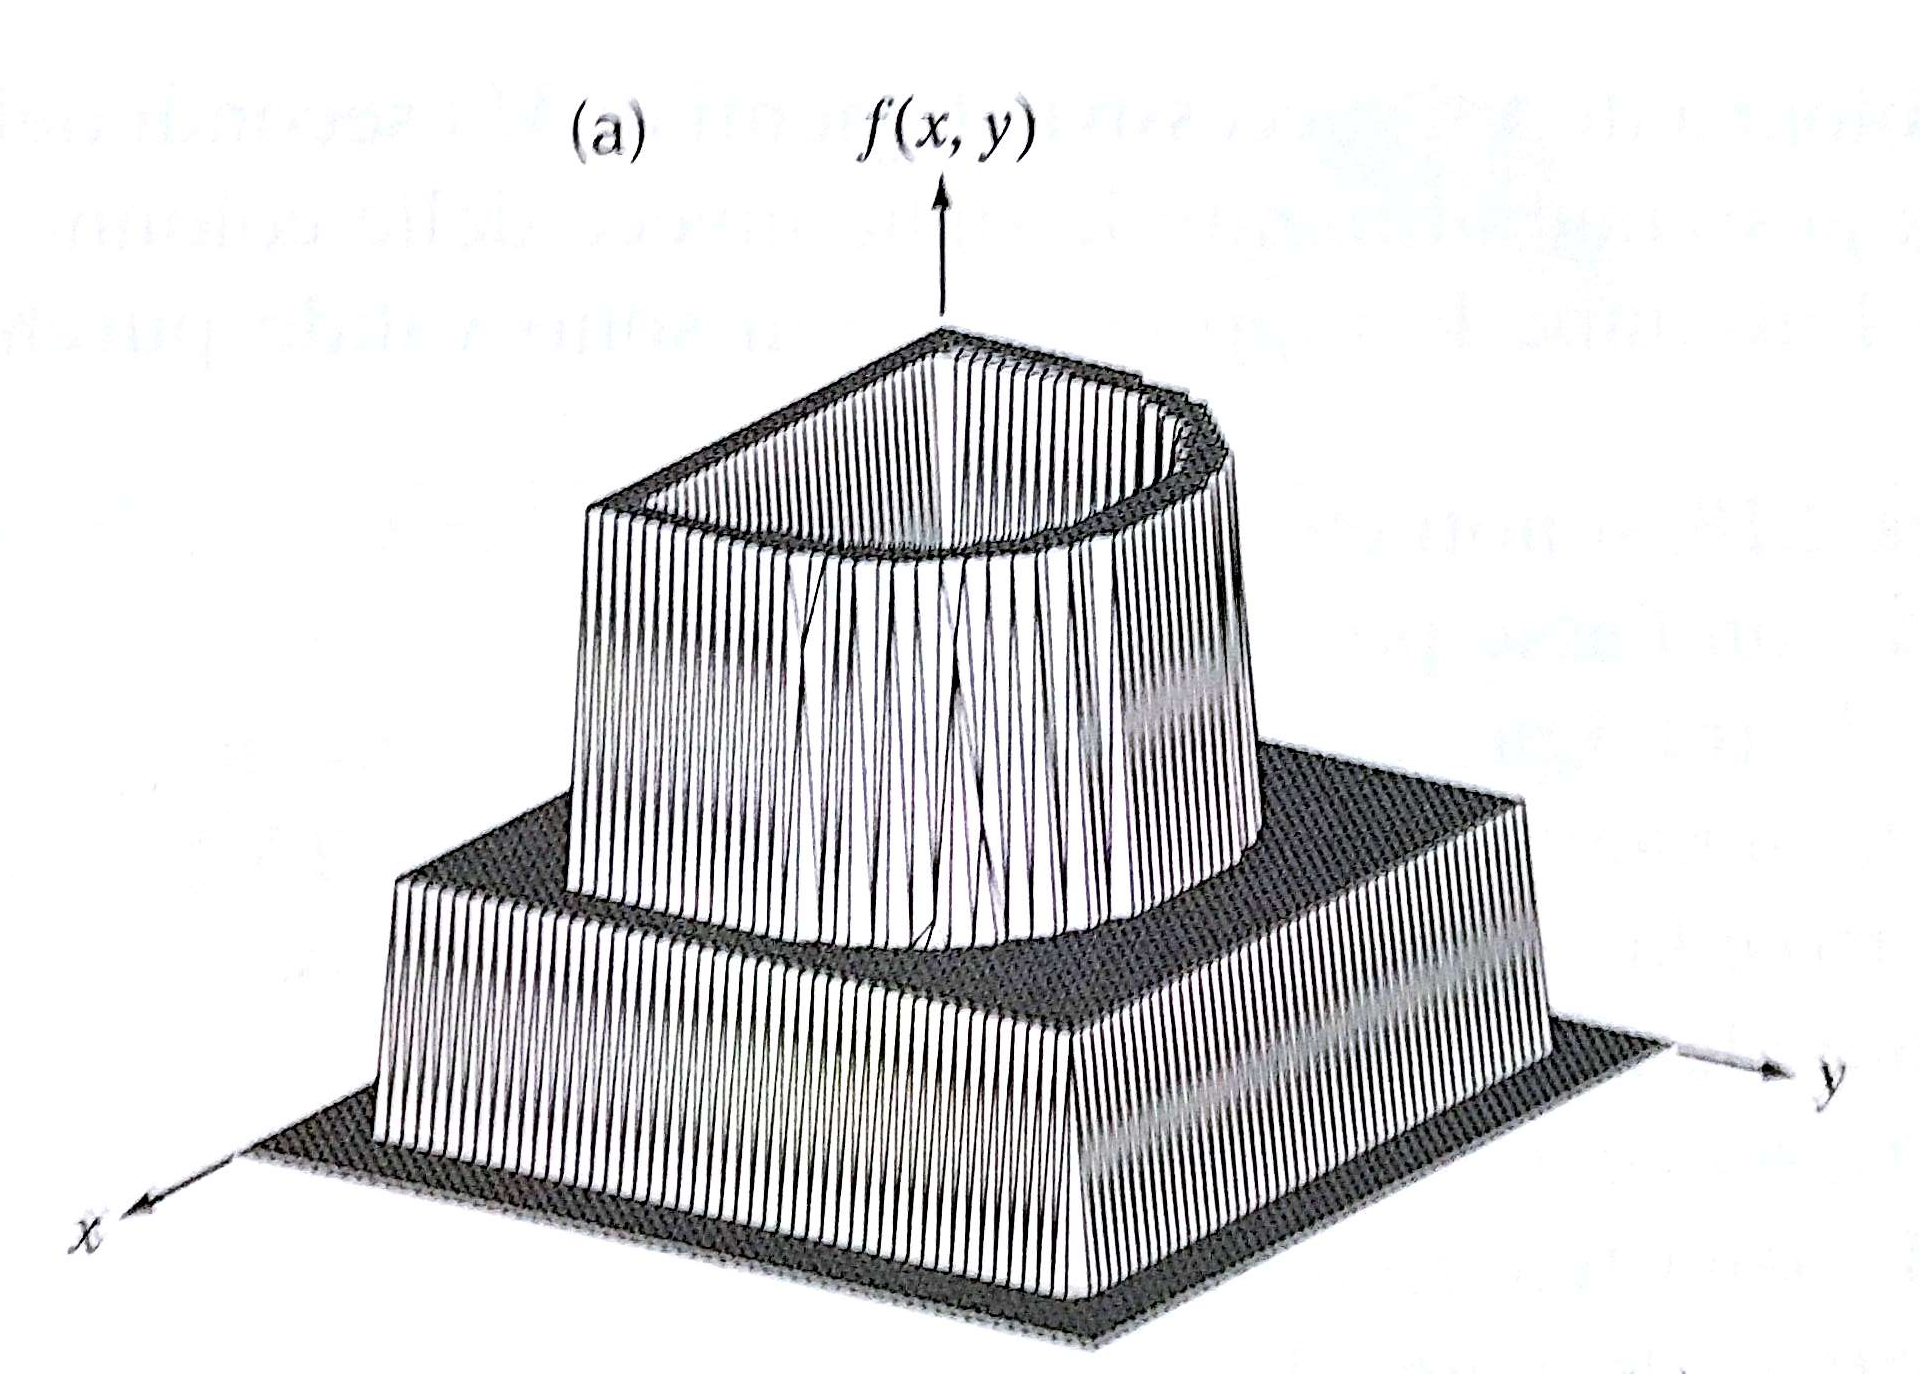
\includegraphics[scale=.15]{img/1050.png}
	\caption{File \protect\url{mission.eps}\label{fig:mission}}
\end{figure}

La segmentazione watershed è utilizzata principalmente per l'estrazione dello sfondo degli oggetti pressoché uniformi (bloblike). Le regioni caratterizzate da piccole variazioni di intensità hanno piccoli valori di gradiente. Per questo motivo si preferisce applicare tale segmentazione al gradiente di una immagine, anziché all'immagine stessa. Nell'esempio che vedremo in seguito, i minimi locali si correlano bene con valori piccoli del gradiente che corrispondono agli oggetti di interesse.

In una topografia consideriamo tre tipi di punti:
\begin{enumerate}
	\item punti appartenenti al minimo locale
	\item punti in cui una goccia d'acqua scorrerebbe verso uno di tali minimi
	\item punti in cui l'acqua potrebbe egualmente cadere in più di un punto di minimo
\end{enumerate}

Per un particolare minimo locale, l'insieme dei punti che soddisfano la condizione 2) è chiamato bacino di raccolta o watershed di questo minimo.

I punti che soddisfano la condizione 3) formano le creste sulla superficie topografica e sono definite linee di divisione o linee di watershed.

Lo scopo dell'algoritmo di segmentazione è quello di trovare le linee di watershed.

Supponiamo che ogni minimo locale venga perforato e che l'intera topografia si riempita dal basso lasciando che l'acqua risalga uniformemente attraverso questi fori.

Quando l'acqua dei differenti bacini rischia di debordare, viene costruita una diga al fine di prevenire tale merging.

L'acqua può raggiungere anche livelli in cui solo le cime di tali dighe risultano visibili. Questi contorni della diga corrispondono alle linee di divisione watershed. Si tratta di contorni connessi estratti dall'algoritmo di segmentazione watershed.

La Fig.10.54 mostra una visualizzazione topografica dell'applicazione dell'algoritmo watershed dove bisogna considerare che:
\begin{itemize}
	\item l'altezza delle "montagne" è proporzionale ai valori di intensità dell'immagine di input
	
	\item per prevenire la crescita del livello dell'acqua oltre i contorni dell'immagine, si chiude il perimetro dell'intera topografia (immagine) con delle dighe che hanno un'altezza maggiore delle montagne, il cui valore viene determinato dal più alto valore possibile di intensità nell'immagine di input
\end{itemize}

\begin{itemize}
	\item si supponga di perforare ogni minimo (le aree in nero in Fig.10.54b) e che l'intera topografia sia sommersa lasciando che il livello dell'acqua risalga da questi buschi a un tasso uniforme
	
	\item la Fig.10.54c mostra un primo livello di inondazione in cui l'acqua (rappresentata in grigio chiaro) ricopre solo le aree che corrispondono allo sfondo nero
	
	\item successivamente, l'acqua risalendo arriva sino ad arrivare rispettivamente al primo e secondo bacino di raccolta (vedi Fig.10.54d e Fig.10.54e)
	
	\item se l'acqua continuasse a salire, questa potrebbe straripare da un bacino all'altro, come accade in Fig.10.54f, dove se non ci fosse una diga (una serie di singoli pixel) l'acqua strariperebbe dal bacino di sinistra a quello di destra
	
	\item in Fig.10.54g l'acqua continua a salire e sono messe in risalto le dighe tra i due bacini e quella in alto del bacino di destra; quest'ultima evita che l'acqua del bacino possa confluire con le aree corrispondenti allo sfondo
	
	\item questo processo continua sino a raggiungere il massimo livello di allagamento corrispondente al valore più alto di intensità dell'immagine
	
	\item la diga finale corrisponde alle linee di watershed, che corrisponde alla segmentazione desiderata come in Fig.10.54h dove si può notare un path di 1 pixel (in nero) sovrapposto all'immagine originale
	
	\item le linee di watershed formano dei path connessi e di conseguenza dei contorni continui tra le regioni
\end{itemize}

\section{L'uso dei marcatori}
L'applicazione diretta dell'algoritmo di segmentazione porta a sovrasegmentazione (oversegmentation) dovuta al rumore o ad altre irregolarità locali del gradiente e questo problema può rendere l'algoritmo di scarsa utilità pratica. Si può migliorare la situazione incorporando una fase di pre-processing (pre-elaborazione) facendo uso per esempio dei marker.

Un marker è una componente connessa appartenente ad una immagine. Si possono avere:
\begin{itemize}
	\item marker interni associati agli oggetti della figura. Una definizione più precisa è:
	\begin{enumerate}
		\item una marker interno è una regione circondata da punti di altitudine elevata
		\item tale che i punti nella regione formino una componente connessa e
		\item in cui tutti i punti della componente connessa abbiamo la stessa intensità
	\end{enumerate}
	
	\item marker esterni associati allo sfondo
\end{itemize}

\subsection{Selezione dei marker}
La tipica procedura per la selezione dei marker consiste di due fasi:
\begin{itemize}
	\item la pre-elaborazione
	\item la determinazione di un insieme di criteri che devono essere soddisfatti dai marker.
\end{itemize}

La selezione del marker può prevedere:
\begin{itemize}
	\item procedure molto semplici basate sui valori di intensità e sulla connettività
	
	\item descrizioni più complesse )
	(dimensione, forma, posizione, distanze relative, tessitura, ecc)
\end{itemize}

L'uso dei marker aggiunge una conoscenza a priori nel processo di segmentazione analoga per certi versi al alcune peculiarità tipiche del sistema visivo umano.

Se consideriamo l'immagine 10.57 noteremo che parte dei problemi sarà dovuta all'eccessiva segmentazione, ovvero di minimi potenziali. A causa della dimensione, molti di questi minimi si riferiscono a dettagli di poco conto. Un metodo efficace per ridurre questo problema, è quello di applicare un filtro di smoothing.

Dopo aver applicato il filtro di smoothing (vedi Fig.10.58a) i marker interni risultanti sono mostrati in grigio chiaro.

In seguito viene applicato l'algoritmo watershed all'immagine con la condizione che \textit{solo} i marker interni siano possibili minimi regionali.

La Fig.10.58a mostra le linee di watershed risultanti e sono definite come marker esterni. Si noti che i punti lungo le linee di watershed passano lungo i punti alti tra i marker vicini.

I marker esterni dividono efficacemente l'immagine in regione, e ognuna di queste contiene un solo marker interno e parte dello sfondo.

A questo punto si possono seguire varie strade:
\begin{itemize}
	\item applicare un qualsiasi algoritmo di segmentazione tra quelli visti in precedenza
	
	\item applicare l'algoritmo di segmentazione ad ogni singola regione. In questo modo si prende in considerazione solo il gradiente dell'immagine e successivamente si applica l'algoritmo solo alle singole watershed che contengono i marker in quella regione.
\end{itemize}

Il risultato finale di buon livello è quello mostrato in Fig.10.58b.
\chapter{Segmentazione Watershed in Matlab}
La trasformata watersher è calcolata dalla funzione $watershed$, la cui sintassi è la seguente:
$$
L = watershed(f)
$$

dove $L$ è una etichetta di matrice con interi positivi che corrispondo ai bacini e con i valori zero usati per indicare le creste watershed.

Uno strumento comunemente utilizzato con la trasformata watershed per la segmentazione è la \textbf{trasformata della distanza}.

La trasformate della distanza di una immagine binaria è la distanza da ogni pixel dal pixel più vicino di valore diverso da zero.

La trasformata della distanza può essere calcolata usando la funzione $bwdist$, la cui sintassi è:
$$
D = bwdist(f)
$$

\section{Segmentazione di una immagine binaria}
\begin{lstlisting}
f = imread('binary-dowel-image.tif');
figure, imshow(f), title('Binary image');

fc = ~f ;
figure, imshow(fc), title('Complement image');

D = bwdist(fc);
figure, imshow(imadjust(uint16(D))), title('Distance transform');

L = watershed(-D);
w = L==0;
figure, imshow(w)
title('Watershed lines of the negative of the distance transform');

g2 = f & ~w ;
figure, imshow(g2)
title('Watershed lines superimposed in black over original binary image');
\end{lstlisting}

\section{Segmentazione di una immagine in toni di grigio}
\begin{lstlisting}
f = imread('small-blobs.tif');
figure, imshow(f), title('Original image');

h = fspecial('sobel');
fd = double(f);
g = sqrt(imfilter(fd, h, 'replicate').^2 + imfilter(fd, h, 'replicate').^2);
figure, imshow(imadjust(uint16(g))), title('Gradient image');

L = watershed(g);
wr = L==0;
figure, imshow(wr), title('Watershed segmentation');

g2 = imclose(imopen(g, ones(3,3)), ones(3,3));
L2 = watershed(g2);
wr2 = L2==0;
f2=f;
f2(wr2)=255;
figure, imshow(f2)
title('Watershed segmentation on smoothed image');
\end{lstlisting}

\section{Segmentazione usando i marcatori}
Per controllare la sovra-segmentazione si utilizzano i marker (marcatori) interni ed esterni.

La funzione IPT $imregionalmin$ calcola la posizione di tutti i minimi locali in una immagine. La sintassi è la seguente:
$$
rm = imregionalmin(f)
$$

dove $f$ è l'immagine in toni di grigio e $rm$ è una immagine binaria in cui i pixel in primo piano marcano le posizioni del minimo locale; questi ultimi possono rappresentare dettagli irrilevanti.

Per eliminare i minimi estranei si utilizza la funzione IPT $imextendedmin$ che calcola l'insieme di punti "bassi" nell'immagine that are deeper than their immediatesurroundings (by a certain height threshold). 

Fornendo sia i marcatori interni che esterni, è possibile modificare l'immagine del gradiente usando una procedura chiamata \textbf{minima imposition}. Questa tecnica modifica una immagine in toni di grigio in modo che i minimi locali si verificano solo nelle posizioni marcate. Altri calori dei pixel sono spinti verso l'alto per rimuovere tutti gli altri minimi locali



\chapter{Image processing con Matlab}

\section{Ridimensionamento}

\textbf{comando:} imresize

\textbf{possibili domande:}
\begin{itemize}
	\item Leggere un'immagine e rimpicciolirla o farne lo zoom di un valore intero
	\item Leggere un'immagine e rimpicciolirla o farne lo zoom di un valore decimale con interpolazione lineare
\end{itemize}

\section{Trasformazioni geometriche}
In Matlab è possibile effettuare una \gls{trasformazione geometrica affine}
specificando la matrice di trasformazione \textit{T} attraverso il comando \textit{maketform}.
Per effettuare la trasformazione si usa il comando \textit{imtransform}.

\textbf{comando:} maketform, imtransform, imrotate, impixelinfo (pixval),

\textbf{possibili domande:}
\begin{itemize}
	\item Effettuare la rotazione di un’immagine qualsiasi
	\item Confrontare il risultato con quello ottenuto mediante la funzione \textit{imrotate}
	\item Leggere l'immagine di 'lena' e realizzare l'ingrandimento di una zona dell’immagine usando la matrice di trasformazione \textit{T}
	la sezione da ingrandire è intorno all'occhio di lena.
	Per individuare la sezione e, quindi, avere informazioni sulla posizione dei pixel potete usare il comando \textit{impixelinfo} o \textit{pixval} (in base alla versione di Matlab più o meno recente).
	\item Fare degli esperimenti modificando il tipo di interpolazione e notate l'effetto di blocchettatura causa
	
	\item La combinazione di diverse trasformazioni affini è ancora una trasformazione 	affine, che può essere ottenuta tramite il prodotto (matriciale) delle matrici che le definiscono.
	
	\item Scrivere una funzione dal prototipo \verb|function g=rot_dist(f, alfa, c)| per realizzare prima una rotazione e poi una distorsione verticale.
	
	\item Creare l'immagine di ingresso usando il seguente comando
	\verb|f = checkerboard(40);| in modo da generare una scacchiera su cui le modifiche risultano essere più facilmente visibili.
\end{itemize}

\section{Rumore}
\begin{itemize}
	\item Aggiungere del rumore gaussiano bianco ad un immagine f con il comando	\verb|noisy = f + n con n = d*randn(size(f))| dove \textbf{d è la deviazione standard del rumore}.
	
	\item Rimuovere il rumore dall'immagine con i filtri a media mobile (al variare della dimensione della finestra).
	
	\item Valutare l'efficacia del filtraggio sia visivamente sia calcolando l'errore quadratico medio tra f e l'immagine "ripulita" .
	
	\item L’errore quadratico medio rappresenta una misura quantitativa per stabilire quanto l'immagine elaborata sia simile all'originale.
	
	\item L'MSE (Mean Squared Error) tra due immagini si definisce come:
	$$
	MSE = {1 \over MN} \sum_{m=0}^{M-1} \sum_{n=0}^{N-1} |f(m, n) - g(m, n)|^2
	$$
\end{itemize}

\section{Smoothing con thresholding}

\begin{itemize}
	\item Consideriamo l'immagine 'telescopio.jpg', proveniente dal telescopio Hubble, in orbita intorno alla terra. Rilevare gli oggetti grandi realizzando le seguenti operazioni:
	\begin{itemize}
		\item Visualizzare l'immagine
		\item Applicare il filtro che effettua la media aritmetica su una finestra di dimensioni 15x15 e visualizzare il risultato
		\item Applicare un'operazione a soglia per eliminare gli oggetti piccoli (considerare una soglia pari al 25 per cento del valore massimo presente nell'immagine filtrata)
		\item Visualizzare il risultato dell'elaborazione
		
	\end{itemize}
\end{itemize}
\chapter{Morfologia Matematica con Matlab}

\section{Introduzione}
Nel contesto dell'image processing l'MM è uno strumento che permette di:

\begin{itemize}
	\item estrarre dall'immagine componenti utili alla rappresentazione e descrizione delle regioni come contorni, scheletri e superfici convessi
	
	\item attuare tecniche particolari come filtri morfologici, thinning e prunning
\end{itemize}

Gli operatori morfologici sono basati sugli \textbf{elementi strutturali} (SE)

\begin{itemize}
	\item gli SE sono piccoli insiemi o sottoimmagini usati per sondare un'immagine per studiarne le proprietà di interesse
	
	\item gli SE, quando lavorano con le immagini sono definiti come array rettangolari
\end{itemize}

\section{Le funzioni MM}

\subsection{strel}
Questa funzione permette di definire gli SE basandosi su diverse forme e dimensioni. La sintassi è:

\begin{lstlisting}
se = strel(shape, parameters)
\end{lstlisting}

\begin{itemize}
	\item \textbf{shape} è una stringa che specifica la forma
	\item \textbf{parameters} è una lista di parametri basati sulla forma scelta, come per esempio la dimensione
\end{itemize}

\subsection{imdilate}
Questa funzione permette la dilatazione secondo la sintassi:

\begin{lstlisting}
IM2 = imdilate(IM, SE)
\end{lstlisting}

\begin{itemize}
	\item \textbf{IM2} è l'immagine in output
	\item \textbf{IM} è l'immagine in input (scala di grigio, binaria)
	\item \textbf{SE} è l'elemento strutturante, o un array di elementi strutturanti restituiti dalla funzione $strel$
\end{itemize}

\subsection{imerode}
Permette l'erosione:

\begin{lstlisting}
IM2 = imerode(IM,SE)
\end{lstlisting}

\begin{itemize}
	\item \textbf{IM2} è l'immagine in output
	\item \textbf{IM} è l'immagine in input (scala di grigio, binaria)
	\item \textbf{SE} è l'elemento strutturante, o un array di elementi strutturanti restituiti dalla funzione $strel$
\end{itemize}

\subsection{imopen}
Questa funzione permette l'opening:

\begin{lstlisting}
IM2 = imopen(IM,SE)
\end{lstlisting}

\subsection{imclose}
Questa funzione permette il closing:

\begin{lstlisting}
IM2 = imclose(IM,SE)
\end{lstlisting}

\subsection{bwhitmiss}
Si tratta della funzione con cui si implementa la trasformazione Hit-or-Miss in base alla sintassi:

\begin{lstlisting}
BW2 = bwhitmiss(BW,SE1,SE2)
\end{lstlisting}

\begin{itemize}
	\item SE1, SE2 sono gli elementi strutturanti
	\item l'operazione Hit-or-Miss preserva i pixel i cui vicini corrispondono alla forma di SE1 e non corrispondono alla forma di SE2
	\item SE1 e SE2 possono essere elementi strutturanti piatti restituiti dalla funzione $strel$ o possono essere array vicini
	
	\item Il dominio di SE1 e SE2 non dovrebbe avere elementi in comune, ovvero:
	
	\begin{lstlisting}
	BW2 = bwhitmiss(BW,SE1,SE2)
	\end{lstlisting}
	
	è equivalente a:
	
	\begin{lstlisting}
	imerode(BW,SE1)
	\end{lstlisting}
	
	e
	
	\begin{lstlisting}
	imerode(~BW,SE2)
	\end{lstlisting}
	
\end{itemize}

\subsection{imfill}
Questa funzione è utilizzata per permettere la copertura di buchi in una immagine binaria, tenendo conto che per buco si intende un insieme di punti dello sfondo che non possono essere raggiunti dal confine dell'immagine. La sintassi è la seguente:

\begin{lstlisting}
BW2 = imfill(BW1,'holes')
\end{lstlisting}

\subsection{bwlabel}
Questa funzione permette di etichettare le componenti connesse in una immagine binaria 2D secondo la sintassi:

\begin{lstlisting}
L = bwlabel(BW,N)
\end{lstlisting}

\begin{itemize}
	\item L è la matrice restituita, della stessa dimensione di BW che contiene l'etichetta per le componenti connesse in BW
	
	\item N può assumere il valore di 4 o 8 corrispondente a oggetti 4-connessi o 8-connessi. Se l'argomento è omesso, il valore di default sarà 8
	
	\item L è un intero che è uguale o maggiore di 0:
	\begin{itemize}
		\item i pixel etichettati con 0 riguardano lo sfondo
		
		\item i pixel etichettati con 1 indicano un oggetto
		
		\item i pixel etichettati con 2 indicano il secondo oggetto e così via
	\end{itemize} 
\end{itemize}

Una seconda sintassi è la seguente:

\begin{lstlisting}
[L, NUM] = bwlabel(BW,N)
\end{lstlisting}

\begin{itemize}
	\item restituisce in NUM il numero di oggetti connessi trovati in BW
\end{itemize}
\chapter{Morfologia matematica binaria}

\section{Funzioni}

\subsection{bwmorph}
Questa funzione implementa diverse operazioni basate sulla combinazione di erosione e dilatazione. La sintassi è:
\begin{lstlisting}
g = bwmorph(f, operation, n)
\end{lstlisting}

\begin{itemize}
	\item $f$ è un'immagina binaria di input
	\item $operation$ è una stringa che specifica le operazioni desiderate
	\item $n$ (opzionale) è un numero intero positivo che indica il numero di volte che l'operazione deve essere ripetuta. Se $n$ viene omesso, l'operazione viene eseguita una sola volta
\end{itemize}

\subsection{imreconstruct}
Implementa la ricostruzione morfologica ed è esplicitata dalla sintassi:
\begin{lstlisting}
out = imreconstruct(marker, mask)
\end{lstlisting}

\begin{itemize}
	\item $marker$ è l'immagine marcatore
	\item $mask$ è l'immagine maschera
\end{itemize}

\subsection{imclearborder}
Permette la pulizia dei bordi degli oggetti, con la sintassi:
\begin{lstlisting}
g = imclearborder(f, conn)
\end{lstlisting}

\begin{itemize}
	\item $f$ è l'immagine di input
	\item $g$ è il risultato
	\item $conn$ può assumere i valori di 4 oppure 8 (valore di default)
\end{itemize}

\section{Esercizi}

\subsection{Esercizio 1}
Calcola e visualizza il centro di massa di ogni componente connesso.
\begin{lstlisting}
f= imread('ten-objects.tif');
imshow(f);
[L, n]=bwlabel(f);
n
hold on; % to plot on the top of the image

for k=1:n
	[r,c] = find(L==k);
	rbar=mean(r);
	cbar=mean(c);
	plot(cbar, rbar, 'Marker', 'o', 'MarkerEdgeColor', 'k', 'MarkerFaceColor', 'k', 'Markersize', 10);
	plot(cbar, rbar, 'Marker', '*', 'MarkerEdgeColor', 'w');
end
\end{lstlisting}

\subsection{Esercizio 2}
Effettua il thinning dell'immagine $finger-print.tif$ sino ad ottenere la stabilità.
\begin{lstlisting}
f=imread('noisy-fingerprint.tif');
imshow(f);
se = strel('square',3);
fo = imopen(f,se);
figure, imshow(fo);
foc = imclose(fo,se);
figure, imshow(foc);

g1 =bwmorph(foc,'thin',1);
figure, imshow(g1);
g2 =bwmorph(foc,'thin',2);
figure, imshow(g2);
ginf =bwmorph(foc,'thin',Inf);
figure, imshow(ginf);
\end{lstlisting}

\subsection{Esercizio 3}
Effettuare la sclettrizzazione dell'immagine $bone$ e si rimuovano i punti finali (5 pixel).
\begin{lstlisting}
f=imread('bone.tif');
imshow(f)
fs = bwmorph(f,'skel',Inf);
figure, imshow(fs);
for k=1:5
	fs=bwmorph(fs,'spur');
end
figure, imshow(fs);
\end{lstlisting}

\subsection{Esercizio 4}
Ricostruzione morfologica
\begin{lstlisting}
marker =imread('recon-marker.tif');
mask = imread('recon-mask.tif');
figure, imshow(mask);
figure, imshow(marker);
recon = imreconstruct(marker, mask);
??? MARKER pixels must be <= MASK
pixels.

Error in ==> imreconstruct at 71
im = imreconstructmex(marker,mask);

mm=marker==255;
mm= uint8(mm*255);
recon = imreconstruct(mm, mask);
figure, imshow(recon);
\end{lstlisting}


\subsection{Esercizio 5}
Effettuare la ricostruzione morfologica per trovare quali caratteri contengono un'asticella verticale.
\begin{lstlisting}
f=imread('book-text.tif');
figure, imshow(f);

fe=imerode(f,ones(51,1));
figure, imshow(fe);

fo=imopen(f, ones(51,1));
figure, imshow(fo);

fobr=imreconstruct(fe,f);
figure, imshow(fobr);
\end{lstlisting}


\subsection{Esercizio 6}
Effettuare una pulizia dei caratteri che toccano lo schermo.
\begin{lstlisting}
g = imclearborder(f);
figure, imshow(g);
figure, imshow(f - g);
\end{lstlisting}
\chapter{Segmentazione Watershed in Matlab}
La trasformata watersher è calcolata dalla funzione $watershed$, la cui sintassi è la seguente:
$$
L = watershed(f)
$$

dove $L$ è una etichetta di matrice con interi positivi che corrispondo ai bacini e con i valori zero usati per indicare le creste watershed.

Uno strumento comunemente utilizzato con la trasformata watershed per la segmentazione è la \textbf{trasformata della distanza}.

La trasformate della distanza di una immagine binaria è la distanza da ogni pixel dal pixel più vicino di valore diverso da zero.

La trasformata della distanza può essere calcolata usando la funzione $bwdist$, la cui sintassi è:
$$
D = bwdist(f)
$$

\section{Segmentazione di una immagine binaria}
\begin{lstlisting}
f = imread('binary-dowel-image.tif');
figure, imshow(f), title('Binary image');

fc = ~f ;
figure, imshow(fc), title('Complement image');

D = bwdist(fc);
figure, imshow(imadjust(uint16(D))), title('Distance transform');

L = watershed(-D);
w = L==0;
figure, imshow(w)
title('Watershed lines of the negative of the distance transform');

g2 = f & ~w ;
figure, imshow(g2)
title('Watershed lines superimposed in black over original binary image');
\end{lstlisting}

\section{Segmentazione di una immagine in toni di grigio}
\begin{lstlisting}
f = imread('small-blobs.tif');
figure, imshow(f), title('Original image');

h = fspecial('sobel');
fd = double(f);
g = sqrt(imfilter(fd, h, 'replicate').^2 + imfilter(fd, h, 'replicate').^2);
figure, imshow(imadjust(uint16(g))), title('Gradient image');

L = watershed(g);
wr = L==0;
figure, imshow(wr), title('Watershed segmentation');

g2 = imclose(imopen(g, ones(3,3)), ones(3,3));
L2 = watershed(g2);
wr2 = L2==0;
f2=f;
f2(wr2)=255;
figure, imshow(f2)
title('Watershed segmentation on smoothed image');
\end{lstlisting}

\section{Segmentazione usando i marcatori}
Per controllare la sovra-segmentazione si utilizzano i marker (marcatori) interni ed esterni.

La funzione IPT $imregionalmin$ calcola la posizione di tutti i minimi locali in una immagine. La sintassi è la seguente:
$$
rm = imregionalmin(f)
$$

dove $f$ è l'immagine in toni di grigio e $rm$ è una immagine binaria in cui i pixel in primo piano marcano le posizioni del minimo locale; questi ultimi possono rappresentare dettagli irrilevanti.

Per eliminare i minimi estranei si utilizza la funzione IPT $imextendedmin$ che calcola l'insieme di punti "bassi" nell'immagine that are deeper than their immediatesurroundings (by a certain height threshold). 

Fornendo sia i marcatori interni che esterni, è possibile modificare l'immagine del gradiente usando una procedura chiamata \textbf{minima imposition}. Questa tecnica modifica una immagine in toni di grigio in modo che i minimi locali si verificano solo nelle posizioni marcate. Altri calori dei pixel sono spinti verso l'alto per rimuovere tutti gli altri minimi locali



\chapter{Le domande da esame}

\section{Immagini digitali}
\begin{itemize}
	\item Image processing, analysis e understanding. Spiegarne la differenza
	\item Definire una immagine digitale
	\item Cosa si intende per risoluzione di una immagine?
	\item Illustrare il processo di campionamento e quantizzazione
	\item Descrivere i passi fondamentali di un processo di elaborazione di immagini digitali
\end{itemize}

\section{Concetti base sulle immagini digitali}
\begin{itemize}
	\item Come si classificano le operazioni spaziali da applicare su un’immagine digitale?
	\item Definire il concetto di adiacenza nelle immagini digitali
	\item Definire una regione di un’immagine binaria
	\item Definire un contorno in un’immagine binaria
	\item Definire un edge in un’immagine digitale
	\item Illustrare il concetto di distanza tra punti in una immagine binaria
	\item Fornire la definizione di istogramma di un’immagine
	\item Illustrare le strutture dati tradizionali per rappresentare un’immagine
	\item Illustrare le strutture dati topologiche per rappresentare un’immagine
	\item Illustrare le strutture dati gerarchiche per rappresentare un’immagine
\end{itemize}

\section{Pre-processing, filtri spaziali, trasformazioni}
\begin{itemize}
	\item Cosa si intende per preprocessing di una immagine
	\item Descrivere i metodi di preprocessing di una immagine
	\item Descrivere le trasformazioni geometriche
	\item Cosa si intende per filtro spaziale?
	\item Cosa si intende per trasformata di una immagine?
	\item Cosa si intende per equalizzazione di un istogramma? A cosa serve?
	\item Come si può realizzare uno stretching del contrasto presente in una immagine?
	\item Definire un filtro spaziale lineare
	\item Cosa si intende per operatore lineare?
	\item Correlazione e convoluzione spaziale. Spiegarne le differenze
	\item Descrivere i filtri per lo smoothing nel dominio spaziale
\end{itemize}

\section{Edge detection}
\begin{itemize}
	\item Illustrare i differenti tipi di edge presenti in un’immagine
	\item Classificazione degli edge detector
	\item Illustrare i metodi per l’edge detection basati sull’approssimazione delle derivate prime.
	\item Descrivere la tecnica della non-maxima suppression
	\item Illustrare il Marr-Hildreth edge detector
	\item Illustrare il Canny edge detector
	\item Quali sono i vantaggi e gli svantaggi degli edge detector?
	\item Quali sono i criteri per valutare la bontà di un edge detector?
	\item Descrivere le tecniche locali e regionali per l’edge linking
	\item Illustrare la trasformata di Hough
\end{itemize}

\section{Segmentazione}
\begin{itemize}
	\item Definizione di segmentazione. Metodi e problemi
	\item Illustrare la segmentazione basata su thresholding
	\item Descrivere il metodo iterativo per la segmentazione mediante soglia globale
	\item Descrivere il metodo per la segmentazione mediante soglia ottimale
	\item Illustrare il metodo region growing per la segmentazione
	\item Illustrare il metodo region splitting and merging per la segmentazione
	\item Descrivere la segmentazione mediante watershed morfologico
\end{itemize}

\section{Descrizione e rappresentazione}
\begin{itemize}
	\item Cosa si intende per rappresentazione e descrizione di un oggetto?
	\item Descrivere i metodi per la rappresentazione del contorno
	\item Illustrare i descrittori del contorno
	\item Illustrare i descrittori semplici di una regione
	\item Illustrare i descrittori topologici di una regione
	\item Illustrare i descrittori basati sulla texture
\end{itemize}

\section{Trasformata di Fourier}
\begin{itemize}
	\item Illustrare la rappresentazione di un’immagine nel dominio spaziale e nel dominio delle frequenze
	\item Fornire la definizione di funzione armonica
	\item Descrivere brevemente la trasformata di Fourier
	\item Quali sono le proprietà della DFT?
	\item Spettro di Fourier, angolo di fase e spettro di potenza. Fornire la loro definizione
	\item Illustrare il teorema di convoluzione
	\item Quali sono i passi da eseguire per il filtraggio nel dominio delle frequenze?
	\item Illustrare la corrispondenza tra filtraggio nel dominio spaziale e filtraggio nel dominio delle frequenze
	\item Descrivere i filtri per lo smoothing nel dominio delle frequenze
	\item Descrivere i filtri per lo sharpening nel dominio delle frequenze
	\item Descrivere i filtri selettivi nel dominio delle frequenze
\end{itemize}

\section{Rumore}
\begin{itemize}
	\item Descrivere il rumore e le sue proprietà
	\item Illustrare i filtri per il rumore (basati sulla media)
	\item Illustrare i ranking filter
	\item Riduzione del rumore periodico mediante filtraggio nel dominio delle frequenze
\end{itemize}

\section{Morfologia matematica}
\begin{itemize}
	\item Cosa è la Morfologia matematica?
	\item In cosa consiste una operazione morfologica?
	\item Fornire la definizione di elemento strutturante nella morfologia matematica
	\item Definire l’erosione e la dilatazione nella morfologia binaria. Illustrarne le proprietà
	\item Definire l’opening e il closing nella morfologia binaria. Illustrarne le proprietà
	\item Definire la trasformazione Hit-or-Miss della morfologia binaria
	\item Come si può realizzare un filtro morfologico?
	\item Illustrare l’algoritmo per l’estrazione del contorno mediante operatori morfologici
	\item Illustrare l’algoritmo per il riempimento di buchi (hole filling) mediante operatori morfologici
	\item Illustrare l’algoritmo per l’estrazione delle componenti connesse mediante operatori morfologici
	\item Illustrare l’algoritmo per l’individuazione della convex hull mediante operatori morfologici
	\item Illustrare l’algoritmo per il thinning mediante operatori morfologici
	\item Illustrare l’algoritmo per il thickening mediante operatori morfologici
	\item Illustrare l’algoritmo per l’estrazione dello skeleton mediante operatori morfologici
	\item Illustrare l’algoritmo per il pruning mediante operatori morfologici
	\item Definire l’erosione e la dilatazione geodesica nella morfologia binaria
	\item Illustrare la ricostruzione morfologica
	\item Illustrare alcune applicazioni della ricostruzione morfologica binaria
	\item Definire l’erosione e la dilatazione nella morfologica in toni di grigio
	\item Definire l’opening e il closing nella morfologia in toni di grigio
	\item Illustrare lo smoothing morfologico
	\item Definire il gradiente morfologico
	\item Descrivere le trasformazioni morfologiche top-hat e bottom-hat
	\item Descrivere la granulometria morfologica
	\item Illustrare la ricostruzione morfologica in tono di grigio
\end{itemize}

\section{Image Processing Toolbox and Matlab}
\begin{itemize}
	\item Quali sono le Data classes per rappresentare un’immagine in Matlab
	\item Quali sono i tipi di immagini supportate da Matlab
	\item Lettura, visualizzazione e salvataggio di immagini in Matlab
	\item Metodi per il miglioramento del contrasto in Matlab
	\item Filtri lineari in Matlab. Come si implementano?
	\item Filtri non lineari in Matlab. Come si implementano?
	\item Edge detection in Matlab. Come si implementa?
	\item Rumore in Matlab. Come si gestisce?
	\item Come si implementa in Matlab la segmentazione mediante soglia?
	\item Descrivere il metodo per il calcolo della DFT 2D in Matlab
	\item Descrivere il metodo per la visualizzazione della DFT 2D in Matlab
	\item Come si crea un elemento strutturante in Matlab?
	\item Descrivere i metodi per realizzare gli operatori morfologici in Matlab
	\item Come si etichettano le componenti connesse in Matlab?
	\item A cosa serve la funzione Matlab bwmorph?
	\item A cosa serve la funzione Matlab imreconstruct?
\end{itemize}

\printindex				% stampa indice analitico

\printglossaries		% stampa glossario
\end{document}